\documentclass[11pt]{amsart}

% --- Packages ---
\usepackage[a4paper,margin=1in]{geometry} % Better for screen reading
\usepackage{amsmath, amssymb, amsthm}    % AMS math packages
\usepackage{hyperref}                    % Clickable references
\usepackage{lipsum}                      % For dummy text (remove later)
\usepackage{tikz}
\usepackage{caption}
\usetikzlibrary{calc,patterns}
\usepackage{setspace}
\usepackage[utf8]{inputenc}
\usepackage[T1]{fontenc}
\usepackage{lmodern}
\usepackage{tcolorbox}
\tcbuselibrary{theorems, breakable, skins, listings}


% --- Theorem Environments ---
\newtheorem{theorem}{Theorem}[section]
\newtheorem{proposition}[theorem]{Proposition}
\newtheorem{lemma}[theorem]{Lemma}
\newtheorem{corollary}[theorem]{Corollary}
\theoremstyle{definition}
\newtheorem{definition}[theorem]{Definition}
\newtheorem{example}[theorem]{Example}

\theoremstyle{remark}
\newtheorem{remark}[theorem]{Remark}

% Unnumbered versions
\newtheorem*{theorem*}{Theorem}
\newtheorem*{proposition*}{Proposition}
\newtheorem*{lemma*}{Lemma}
\newtheorem*{corollary*}{Corollary}
\newtheorem*{definition*}{Definition}
\newtheorem*{example*}{Example}
\newtheorem*{remark*}{Remark}
\newtheorem*{claim}{Claim}


% --- Lecture counter ---
\newcounter{lecture}
\renewcommand{\thelecture}{\arabic{lecture}}
\makeatletter
\renewcommand{\theHsection}{\thelecture.\arabic{section}}
\renewcommand{\theHsubsection}{\thelecture.\arabic{section}.\arabic{subsection}}
\renewcommand{\theHsubsubsection}{\thelecture.\arabic{section}.\arabic{subsection}.\arabic{subsubsection}}
\makeatother
% Make sections depend on lecture
\renewcommand{\thesection}{\thelecture.\arabic{section}}
\newcommand{\lecture}[1]{%
  \refstepcounter{lecture}%
  \bigskip\hrule\bigskip
  {\Large\bfseries Lecture \thelecture: #1 \par}\medskip
  \addcontentsline{toc}{chapter}{Lecture \thelecture: #1}%
  \setcounter{section}{0} % reset sections for each lecture
}

% --- Metadata ---
\title{Lecture Notes in Mathematics}
\author{Zian Gong}
\date{\today}

\begin{document}

\maketitle
\tableofcontents

\setlength{\parskip}{0.8em}   % 段落之间距离
\setlength{\parindent}{2em}   % 段首缩进
% % 1.5 倍行距
\onehalfspacing

% % 双倍行距
% \doublespacing

% 或者手动指定,比如 1.2 倍
% \setstretch{1.2}



\newpage
\lecture{Univariate Analysis}

\begin{definition}[Commodity Bundles and Constraints]
    Budget Set = consumption set + economic constrains \[
        \beta(p,w) = \{x \in X: px \leq w\}
    \] where:
    \begin{itemize}
        \item $p = (p_1, p_2,\dots,p_L) \in \mathbb{R}^{L}$ is a price vector,
        \item $w \in \mathbb{R}^{+}$ is wealth,
        \item Consumption Plans: $x = (x_1, x_2, \dots, x_L) \in \mathbb{R}^{L}$,  $\left\{\begin{array}{l}
                      x_l > 0: \text{receive}   \\
                      x_l < 0: \text{give away} \\
                  \end{array}\right.$
        \item Consumption Set: $X \in \mathbb{R}^{L}$, in general we assume $X = \mathbb{R}^{L}_{+}\equiv\{x\in \mathbb{R}^{L}: x \geq 0\}$
        \item  Commodity Space $\mathbb{R}^{L}$: finite number of goods, perfect divisibility.
    \end{itemize}

\end{definition}
\begin{remark*}
    Implicit Assumptions: \begin{itemize}
        \item Price-taking consumers
        \item Perfect Information
        \item Complete Markets
        \item Exogenous Wealth
        \item Linear Budget Constraint
    \end{itemize}

    Normally, budget set is \textbf{compact} and \textbf{convex}, and $p \gg 0$.
    A counterexample: quantity discount.
\end{remark*}

\section{Preference}
\begin{definition}[Preference]
    \textbf{Preference} is represented by $\succeq$, a binary relationship on $X$: \[
        (X, \succeq) \subset X \times X: x^{1} \succeq x^{2} \iff(x^{1}, x^{2}) \in (X, \succeq)
    \] which means $x^{1}$ is at least as good as $x^{2}$.
    \begin{remark*}
        $X$ represents the consumption set, $X \times X$ is the \underline{Cartesian Product}, which represents all the possible combo pairings of commodities. $(x^{1}, x^{2})$ represents an \underline{Ordered Pair}.
    \end{remark*}

    \textbf{Strict Preference} $\succ$: \[
        x^{1} \succ x^{2} \iff x^{1} \succeq x^{2} \wedge \neg(x^{2} \succeq x^{1})
    \]

    \textbf{Indifference} $\sim$: \[
        x^{1} \sim x^{2} \iff x^{1} \succeq x^{2} \wedge x^{2} \succeq x^{1}
    \]
\end{definition}

Properties of \textbf{rational preferences}: \begin{enumerate}
    \item Transitivity: $\forall x^{1}, x^{2}, x^{3} \in X$: $ x^{1} \succeq x^{2} \wedge  x^{2} \succeq x^{3} \Longrightarrow  x^{1} \succeq x^{3}$.
    \item Completeness: $\forall x^{1}, x^{2} \in X \Longrightarrow x^{1} \succeq x^{2} \vee x^{2} \succeq x^{1}$.
\end{enumerate}
Other preference properties:
\begin{enumerate}
    \setcounter{enumi}{2}
    \item Continuity: $\forall x^{0} \in X$, the sets $\{x \in X: x \succeq x^{0}\}$ and $\{x \in X: x^{0} \succeq x\}$ are closed. \begin{itemize}
              \item Upper Contour Set and Lower Contour Set are closed.
              \item $\succeq$ is continuous $\iff \forall x^{0} \in X, $ an arbitrary convergent sequence $(x^{n})^{\infty }_{n=1}$, \[
                        \Big[\forall n, x^{n} \succeq x^{0}\Big] \Longrightarrow \Big[\lim_{n \to \infty} x^{n} = x \succeq x^{0}\Big]
                    \] \[
                        \Big[\forall n, x^{0} \succeq x^{n}\Big] \Longrightarrow \Big[\lim_{n \to \infty} x^{n} = x,\, x^{0} \succeq x\Big]
                    \]
                    A counterexample is the \underline{Lexicographic Order} in $\mathbb{R}^{2}_{+}$: \[
                        x \succeq x^{0} \iff (x_1 > x_1^0) \wedge (x_1=x_1^0 \wedge x_2 \geq x_2^0)
                    \], e.g., $x^{0}=(5,2), x^{n} = (5+1/n,0)$ for any $n$, we have $5+1/n > 5 \Longrightarrow x^{n} \succeq x^{0}$, however, $\lim_{n \to \infty} x^{n} = (5,0) \nsucceq x^{0}$.
              \item Closed Set: A set $A$ is closed iff all convergent sequence in $A$ has their limits in $A$.
          \end{itemize}
    \item Local nonsatiation: $\forall x^{0} \in X, \forall \varepsilon > 0, \exists x^{1} \in X \Longrightarrow ||x^{0}-x^{1}||<\varepsilon \wedge x^{1} \succ x^{0}$ \begin{itemize}
              \item It means we can always find a direction to improve.
          \end{itemize}
    \item[(4')] Monotonicity: $\forall x^{0}, x^{1}: x^{1} \gg x^{0} \Longrightarrow x^{1} \succ x^{0}$. (All goods more than initial set)
    \item[(4'')] Strong Monotonicity: $\forall x^{0}, x^{1}, x^{1} \neq x^{0}: x^{1} \geq x^{0} \Longrightarrow x^{1} \succ x^{0}$. (Some goods more than initial set) \begin{itemize}
              \item We can prove (4'') $\Longrightarrow$ (4') $\Longrightarrow$ (4).
          \end{itemize}
    \item Convexity: $\forall x \in X, \{x \in X: x \succeq x^0\}$ is convex. \begin{itemize}
              \item The upper contour set is convex.
              \item Convexity also gives the information about how the MRS changes while increasing one good.
              \item $(3)+(4)+(5) \Longrightarrow$ a nice indifference curve: \begin{enumerate}
                        \item Continuity gives us a solid, unbroken line.
                        \item Monotonicity makes that line slope downwards from left to right.
                        \item Convexity bends that downward-sloping line so it's bowed in toward the origin.
                    \end{enumerate}
          \end{itemize}
    \item[(5')] Strict Convexity: $\forall \lambda \in (0,1)\, \forall x^0,x^1,x^2 \in X: x^1 \neq x^2, x^1 \succeq x^0 \Longrightarrow \lambda x^1 + (1-\lambda)x^2 \succ x^0$. \begin{itemize}
              \item It's just a strict version of $(5)$.
          \end{itemize}
\end{enumerate}

\section{Utility Function}

\begin{definition}
    Given a rational preference $\succeq $ on $X$. A \textbf{utility function} $u: X \longrightarrow \mathbb{R}$ that represents $\succeq $ is such that \[
        \forall x^0,x^1 \in X, x^0 \succeq x^1 \iff u(x^0) \geq u(x^0).
    \]
\end{definition}

\begin{proposition}
    \[
        \left\{\begin{array}{l}
            x^0 \succ x^1 \iff u(x^0) > u(x^1) \\
            x^0 \sim x^1 \iff u(x^0) = u(x^1)  \\
        \end{array}\right.
    \]
\end{proposition}

\begin{proposition}[ordinality]
    Given $u: X \longrightarrow \mathbb{R}$ representing $\succeq $ and $f: \mathbb{R} \longrightarrow \mathbb{R}$ any strict increasing function, then $v = f \circ u$ also represents $\succeq $.
\end{proposition}

\begin{proof}
    $\forall x^0,x^1 \in X, x^0 \succeq x^1$.

    $u$ represents $succeq$: $u(x^0) \geq u(x^1)$

    $f$ is strictly increasing: $f(u(x^0)) \geq f(u(x^1)) \iff v(x^1) \geq v(x^0)$
\end{proof}

\begin{remark*}
    The "ordinality" implicitly means the scale of the utility function means nothing.
\end{remark*}

\begin{theorem}[Debreu's]
    Given a \textbf{rational preference} $\succeq$ on $X \subset \mathbb{R}^{L}_{+}$. If $\succeq $ is \textbf{continuous}, then there \textbf{exists} a \underline{continuous utility function} $u: X \longrightarrow \mathbb{R}$ that represents $\succeq $.
\end{theorem}

\begin{proof}
    To give a simple and intuitive proof, we assume $X = \mathbb{R}^{L}_{+}$, and that the preference $\succeq$ is also \textbf{monotone}.

    The proof proceeds by construction. We define a function $u(x)$ by mapping each bundle $x$ to a specific amount of a reference bundle, $e=(1,\dots,1)$. We then show this function is well-defined, represents the preferences, and is continuous.

    \textbf{Step 1:} The utility function $u(x)$ is well-defined

    For any bundle $x \in \mathbb{R}^L_+$, we must show there exists a \textbf{unique} scalar $\lambda_x \ge 0$ such that $\lambda_x e \sim x$.

    To do this, we define the set $F_x = \{\lambda e : \lambda \geq 0, \lambda e \preceq x \}$. This set contains all bundles on the main diagonal that are weakly inferior to $x$. We will show this set is compact (closed and bounded) and non-empty.

    \begin{itemize}
        \item[\textit{(1)}] \textit{\underline{Proof of non-empty:}} The zero bundle $\mathbf{0} = 0 \cdot e$. By monotonicity, $x \succeq \mathbf{0}$ for any $x \in \mathbb{R}^L_+$. Thus, $0 \cdot e \in F_x$, and $F_x$ is not empty.

        \item[\textit{(2)}] \textit{\underline{Proof of bounded:}} By monotonicity, for any $x \in \mathbb{R}^L_+$, we can find a bundle $z$ such that $z \gg x$ (e.g., $z_i = x_i + 1$ for all $i$), which implies $z \succ x$. Now, for a sufficiently large scalar $\bar{\lambda}$, we will have $\bar{\lambda} e \gg z$. Monotonicity then implies $\bar{\lambda} e \succ z$. By transitivity, $\bar{\lambda} e \succ x$. This means that any vector $\lambda e \in F_x$ (where $\lambda e \preceq x$) must have its components bounded by those of $\bar{\lambda}e$. Thus, the set of vectors $F_x$ is bounded.

        \item[\textit{(3)}] \textit{\underline{Proof of closed:}} The set $F_x$ is the intersection of the ray $R = \{\lambda e : \lambda \ge 0\}$ and the lower contour set $LCS_x = \{y \in \mathbb{R}^L_+ : y \preceq x\}$. The ray $R$ is a closed set. Because the preference relation $\succeq$ is \textbf{continuous}, the set $LCS_x$ is also closed. The intersection of two closed sets is closed, therefore $F_x$ is closed.
    \end{itemize}

    Since $F_x$ is a non-empty, closed, and bounded subset of $\mathbb{R}^L_+$, it is \textbf{compact}.

    Now, consider the function $f: F_x \to \mathbb{R}$ defined by $f(\lambda e) = \lambda$. This function is continuous. By the \textbf{Weierstrass Extreme Value Theorem}, a continuous function on a compact set attains its maximum. Let this maximum value be $\lambda^*$, achieved at the point $\lambda^* e \in F_x$.

    By construction, since $\lambda^* e \in F_x$, we know $\lambda^* e \preceq x$.

    We must also show $\lambda^* e \succeq x$. We prove this by contradiction. Assume $\lambda^* e \prec x$. This means $\lambda^* e$ is in the \textbf{strict lower contour set} of $x$, $SLCS_x = \{y \in X : y \prec x\}$. Since $\succeq$ is continuous, the set $SLCS_x$ is \textbf{open}.

    Because $\lambda^* e \in SLCS_x$ and $SLCS_x$ is open, there exists an $\varepsilon > 0$ such that the bundle $(\lambda^* + \varepsilon)e$ is also in $SLCS_x$. This means $(\lambda^* + \varepsilon)e \prec x$, which in turn implies $(\lambda^* + \varepsilon)e \preceq x$. By definition, this means $(\lambda^* + \varepsilon)e \in F_x$.

    However, this implies that the function $f(\lambda e) = \lambda$ attains the value $\lambda^* + \varepsilon$ on the set $F_x$. This contradicts $\lambda^*$ being the maximum value of $f$ on $F_x$.

    Therefore, the assumption $\lambda^* e \prec x$ must be false. Since we have both $\lambda^* e \preceq x$ and $\neg(\lambda^* e \prec x)$, we conclude that $\lambda^* e \sim x$. Uniqueness of $\lambda^*$ follows from strict monotonicity.

    We can now define the utility of $x$ as this unique scalar: $u(x) \doteqdot \lambda^*$.

    \textbf{Step 2:} $u(x)$ represents $\succeq$

    We must prove that for any $x, y \in X$, we have $x \succeq y \iff u(x) \geq u(y)$.

    ($\Longrightarrow$) Assume $x \succeq y$. By definition of our function, we have $x \sim u(x)e$ and $y \sim u(y)e$.
    By transitivity, the relations $x \succeq y$ and $x \sim u(x)e$ imply $u(x)e \succeq y$.
    Again by transitivity, $u(x)e \succeq y$ and $y \sim u(y)e$ imply $u(x)e \succeq u(y)e$.
    By monotonicity, for bundles on the main diagonal, $u(x)e \succeq u(y)e$ holds if and only if $u(x) \geq u(y)$.

    ($\Longleftarrow$) Assume $u(x) \geq u(y)$.
    By monotonicity, this implies $u(x)e \succeq u(y)e$.
    By definition, we have $x \sim u(x)e$ and $y \sim u(y)e$.
    Using transitivity on the entire relation: $x \sim u(x)e \succeq u(y)e \sim y$. This implies $x \succeq y$.

    \textbf{Step 3:} $u(x)$ is continuous

    \textbf{A real-valued function is continuous if and only if the inverse images of all closed intervals are closed sets.} ("A real-valued function is continuous if and only if the inverse images of all open intervals are open sets." is also correct.) This is equivalent to showing that for any scalar $\bar{\lambda}$, the sets $\{x \in X : u(x) \geq \bar{\lambda}\}$ and $\{x \in X : u(x) \leq \bar{\lambda}\}$ are both closed.

    (a) Consider the set $A = \{x \in X : u(x) \geq \bar{\lambda}\}$. From Step 2, the condition $u(x) \geq \bar{\lambda}$ is equivalent to $x \succeq \bar{\lambda}e$. Thus, $A = \{x \in X : x \succeq \bar{\lambda}e\}$. This is, by definition, the \textbf{upper contour set} of the bundle $\bar{\lambda}e$. By the initial assumption that the preference relation $\succeq$ is continuous, all its upper contour sets are closed. Therefore, $A$ is a closed set.

    (b) Consider the set $B = \{x \in X : u(x) \leq \bar{\lambda}\}$. Similarly, the condition $u(x) \leq \bar{\lambda}$ is equivalent to $x \preceq \bar{\lambda}e$. Thus, $B = \{x \in X : x \preceq \bar{\lambda}e\}$. This is the \textbf{lower contour set} of the bundle $\bar{\lambda}e$. Since $\succeq$ is continuous, all its lower contour sets are also closed. Therefore, $B$ is a closed set.

    Since both the upper and lower contour sets of the function $u(x)$ are closed for any value in its range, the function $u(x)$ is \textbf{continuous}.
\end{proof}

\begin{proposition}
    Given preference $\succeq $ with a utility representation $u$, we have that: \begin{align*}
        \succeq \text{continuous}          & \iff \text{there exists $u'$ continuous representing $\succeq $} \\
        \succeq \text{locally nonsatiated} & \iff \text{$u$ has no local maxima}                              \\
        \succeq \text{strongly monotone}   & \iff \text{$u$ is strictly increasing}                           \\
        \succeq \text{(strict) convex}     & \iff \text{$u$ is strict quasiconcave}                           \\
    \end{align*}
\end{proposition}


\section{Walrasian Demand and Indirect Utility}

\begin{definition}
    For program [P] \begin{align*}
         & \max_{x \in X} u(x)      \\
         & s.t. \, x \in \beta(p,w)
    \end{align*}

    \textbf{Indirect Utility}: $v(p,w) \equiv \max_{x \in \beta(p,w)} u(x)$.

    \textbf{Walrasian Demand}: $x(p,w) \equiv \arg\max_{x \in \beta(p,w)} u(x)$.

\end{definition}

\begin{remark*}
    $v(p,w)$ is also called value function, while $x(p,w)$ is a correspondence.

    Difference between "function" and "correspondence": \begin{itemize}
        \item Function: one input only maps to one output.
        \item Correspondence: one input maps to a set of outputs.
    \end{itemize}
\end{remark*}

\begin{proposition}
    If $u(\cdot )$ is continuous, then for any $p \gg 0$ and $w \geq 0$ the program [P] \textbf{has a solution}.

    If $u(\cdot )$ is also strictly quasiconcave, then the solution is \textbf{unique}. Moreover, $x(p,w)$ is a continuous function.
\end{proposition}

\begin{proof} Existence and Uniqueness.

    Existence: (Weierstrass Theorem): $u(\cdot )$ is continuous and $\beta(p,w)$ is compact $\Longrightarrow$ exists a maxima.

    Uniqueness: By contradiction: $\exists x^1, x^2 \in X: x^1, x^2 \in \beta(p,w) $ and $u(x) \leq u(x^1), u(x)\leq u(x^2)\, \forall x \in \beta(p,w)$. Then we have $u(\lambda x^1 + (1-\lambda)x^2) > \min\{u(x^1), u(x^2)\} \Longrightarrow u(x') > u(x^1)$. It contradicts to $u(x) \leq u(x^1)\, \forall x \in \beta(p,w)$.
\end{proof}
\newpage
\lecture{Linear Algebra}

\begin{definition}[Experiment of chance]
    It is an experiment that can be repeated under the same conditions, where the exact outcome is uncertain before it occurs, but the set of all possible outcomes is known.
\end{definition}

\begin{definition}[Probability space]
    A formal mathematical model of the experiment of chance.
\end{definition}

\begin{definition}
    The \textbf{sample space} (usually denoted by $S$ or $\Omega$) is the set of all possible outcomes of an experiment of chance.
\end{definition}
\begin{example*}
    \[
        S = \{ \text{Heads}, \text{Tails} \} \quad \text{(coin toss)}
    \]
    \[
        S = \{1, 2, 3, 4, 5, 6\} \quad \text{(roll a die)}
    \]
\end{example*}

\begin{definition}
    An \textbf{event} (denoted by $B$) is any subset of the sample space. It represents one or more outcomes of interest.
\end{definition}
\begin{example*}
    Examples (rolling a die):
    \[
        A = \{2,4,6\} \quad \text{(event: ``even number'')}
    \]
    \[
        B = \{5,6\} \quad \text{(event: ``greater than 4'')}
    \]

    Example (tossing a coin):
    \[
        C = \{\text{Heads}\} \quad \text{(event: ``get Heads'')}
    \]

\end{example*}

\subsection*{Event Space}
The \textbf{event space} (denoted by $\mathcal{B} $ or $ \mathcal{F}$) (also called a $\sigma$-algebra) is the collection of all events that are measurable in a probability model.
It must satisfy:
\begin{enumerate}
    \item $\Omega \in \mathcal{B}$ (the sample space is included),
    \item $\varnothing \in \mathcal{B}$ (the empty set is included),
    \item If $A \in \mathcal{B}$, then $A^c \in \mathcal{B}$ (closed under complementation),
    \item If $A_1, A_2, \dots \in \mathcal{B}$, then $\bigcup_{i=1}^\infty A_i \in \mathcal{B}$ (closed under countable unions).
\end{enumerate}
\begin{example*}
    Example (coin toss once):
    \[
        S = \{H, T\}, \quad
        \mathcal{B} = \{\varnothing, \{H\}, \{T\}, \{H,T\}\}
    \]
\end{example*}

\begin{definition}[A probability measure $p()$] A function which maps $B$ onto $[0,1]$ according to certain rules of Axioms of Probability.
    % Properties: \begin{enumerate}
    %     \item $ p(A) \geq 0, \forall A \in B$
    %     \item $p(\omega ) = 1$
    %     \item $\{A_i, i = 1,2,\dots\}$ be a collection of pairwise disjoint events $p(\bigcup_i A_i) = \sum_{i}^{} p(A_i)$
    %     \item 
    % \end{enumerate}
\end{definition}

\section{Random variable}

\begin{definition}
    A \textbf{random variable} $X$ can be fully characterized by means of a \textbf{cumulative distribution function (cdf)} $F_x$, a function which gives the probabilities of events of the form $X \leq x$ for all $x$. \[
        F_x : \mathbb{R} \to [0,1],\, F_X(x) \equiv p(X \leq x).
    \]
\end{definition}

Properties of a cdf: \begin{itemize}
    \item $F(-\infty ) = 0, \, F(\infty ) = 1$.
    \item $F$ is non-decreasing.
    \item $F$ is right-continuous.
\end{itemize}

\section{Discrete and continuous random variables}

\textbf{Discrete random variable}: $X$ is discrete if its range (support) is a finite or countable set. \begin{itemize}
    \item The cdf is a step function.
    \item $p(X=x_i)$ is the \textbf{probability mass function (pmf)} and $\sum_{i=1}^{} p_i = 1$.
\end{itemize}


\textbf{Continuous random variable}: The random value $X$ with cdf $F(\cdot )$ is continuous if there exists a (non-negative) function $f(\cdot )$, which is call the probability \textbf{density} function (\textbf{pdf}), such that \[
    F(x) = \int_{-\infty }^{x}f(z) \, dz
\]

Properties if the cdf and pdf of continuous random variables: \begin{itemize}
    \item $f(x) \geq 0$ at all points where $F(\cdots )$ is differentiable.
    \item $\int_{-\infty }^{\infty } f(z) \, dz = 1$.
    \item $F$ is continuous.
    \item $p(X=b) = 0$.
    \item $p(a<X<b) = \int_{a}^{b} f(z) \, dz$.
\end{itemize}

\begin{remark*}
    $f(\cdot )$ represents the probability in a unit length of interval.
    $f(\cdot )$ can be larger than $1$ in a very small interval.
\end{remark*}

\textbf{Mixed variables} \[
    F(x) = pF_d(x) + (1-p)F_c(x), \, 0 < p < 1, F_d \text{ is discrete and } F_c \text{ is continuous}
\]
\begin{remark*}
    How to understand mixed variables: Think about 2 stages:

    Wages: $20\%$ unemployed and $80\%$ employed. In those who are employed, $40\%$ worker's wages are less than $1000$, $60\%$'s wages are less than $3000$, and $100 \%$'s wages are less than $5000$. \[
        \text{wages} = \left\{\begin{array}{l}
            \text{unemployed } 20\% \Rightarrow w = 0 \\
            \text{employed } 80\% \Rightarrow \left\{\begin{array}{l}
                                                         40\% \Rightarrow 0 < w \leq 1000  \\
                                                         60\% \Rightarrow 0 < w \leq 3000  \\
                                                         100\% \Rightarrow 0 < w \leq 5000 \\
                                                     \end{array}\right.
        \end{array}\right.
    \]

    What is the probability of a random people's wage is under $3000$? We should calculate: \[
        p(w \leq 3000)  = 20\% \times 1 + 80\% \times 60\% = 68\%
    \]
\end{remark*}


\section{Univariate normal distribution}

\begin{definition}
    \textbf{Standard Normal} $N(0,1)$. \begin{itemize}
        \item pdf: $\phi (x) = \frac{1}{\sqrt{2 \pi }} \exp(-\frac{x ^{2}}{2})$ \begin{itemize}
                  \item $\phi (x) $ is symmetric about $0$.
                  \item $\phi (x) $ has a unique maximum at $x = 0$.
                  \item $\phi (x)$ has two inflexion points at $\pm 1$
              \end{itemize}
        \item cdf: $\Phi(x) = \int_{-\infty }^{x} \phi (z) \, dz$
    \end{itemize}
\end{definition}

\begin{definition}
    \textbf{Normal family} $N(\mu, \sigma^2)$. Let $Z \sim N(0,1), X \equiv \mu + \sigma Z$ with $\sigma > 0$, then $X \sim N(\mu, \sigma^2)$. \begin{itemize}
        \item cdf: $F_X(x) = \Phi(\frac{x-\mu}{\sigma})$
        \item pdf: $f_X(x) = \frac{1}{\sigma}\phi(\frac{x-\mu}{\sigma})$ \begin{itemize}
                  \item $f_X(\cdot )$ is symmetric about $\mu$.
                  \item $\phi (x) $ has a unique maximum at $x = \mu$.
                  \item $\phi (x)$ has two inflexion points at $\mu \pm \sigma$.
              \end{itemize}
    \end{itemize}
\end{definition}


\section{Functions of random variables}

\subsection{Discrete case} $y_i= g(x_i)$:
\[
    p(Y=y) = \sum_{i: g(x_i)=y}^{} p(X=x_i)
\]

\subsection{Continuous case} $Y = g(X)$, if $g$ is continuous and differentiable, $g'\neq 0$ \[
    f_Y(y) = \left| \frac{dx}{dy}\right| f_X(g^{-1}(y)) , \, \frac{dx}{dy} = \frac{1}{g'[g^{-1}(y)]}
\]

\begin{proof}
    \begin{align*}
         & F_Y(y) \equiv p(Y \leq y) = p(X \leq g^{-1}(y)) = F_X(g^{-1}(x)) \\
         & f_Y(y) = \frac{d F(x)}{dy} = \frac{dx}{dy} f_X(g^{-1}(y))
    \end{align*}
    But $\frac{dx}{dy}$ should be the absolute value because $f(\cdot) \geq 0$.
\end{proof}

\newpage
\lecture{Analysis in $\mathbb{R}^{n}$}
% TeX root = ../Main.tex
% First argument to \section is the title that will go in the table of contents. Second argument is the title that will be printed on the page.

\section{Metric Space}

\begin{definition}
    A set $X$ is said to be a \textbf{\textit{metric space}} if $\forall p,q \in X$, there is an associated real number $d(p,q)$ called the distance from $p$ to $q$ such that:
    \begin{itemize}
        \item $d(p,q)>0$ if $p \neq q$ and $d(p,q) = 0$ if $p=1$,
        \item $d(p,q) = d(q,p)$, and
        \item $d(p,q) \leq d(p,r) + d(r,q), \forall r \in X$ (Triangle Inequality).
    \end{itemize}
\end{definition}

\begin{remark*}
    Any function with these properties is called a \textbf{\textit{distance function}} or a \textbf{\textit{metric}}.
\end{remark*}

\section{Euclidean Space}

We can define the following operations in $\mathbb{R}^{n}$:

\begin{definition}[\textbf{Sum}]
    Given $\mathbf{x, y} \in \mathbb{R}^{n}, x+y = (x_{1}+y_{1}, \dots,x_{n}+y_{n})' \in \mathbb{R}^{n}$
\end{definition}

\begin{definition}[\textbf{Scalar Multiplication}]
    Given $a \in \mathbb{R}$ and $\mathbf{x} \in \mathbb{R}^{n}, a \mathbf{x} = (ax_1,\dots,ax_n)' \in \mathbb{R}^{n}$
\end{definition}

\begin{definition}[\textbf{Inner Product}]
    Given $\mathbf{x, y} \in \mathbb{R}^{n}, x\cdot y = \sum_{i=1}^{n} x_{i}y_{i} \in \mathbb{R}^{n}$
\end{definition}

\begin{remark*}[Vector Space]
    With operations "Sum" and "Scalar Multiplication", we can say that $\mathbb{R}^{n}$ is a \textbf{Vector Space}. \textit{(See the Definition in Section "Vector Space and Subspace")}
\end{remark*}

\begin{remark*}[Euclidean Space]
    With operations "Sum", "Scalar Multiplication" and "Inner Product" make $\mathbb{R}^{n}$ a \textbf{Euclidean Space}.
\end{remark*}

\begin{definition}[Euclidean Norm]
    The \textbf{Euclidean Norm} of a vector $\mathbf{x} \in \mathbb{R}^{n}$ is given by \begin{equation*}
        ||\mathbf{x}||=\sqrt{\mathbf{x}\cdot \mathbf{x}} = \sqrt{\sum_{i=1}^{n} x^2_{i}}.
    \end{equation*}
\end{definition}

\begin{definition}[$p$-Norm*]
    \begin{equation*}
        ||\mathbf{x}||_p = \Big(\sum_{i=1}^{n} |x_i|^p\Big)^{1/p}, \quad p \geq 1
    \end{equation*}
    \begin{remark*}
        Euclidean norm is a spacial case of the $p$-norm with $p=2$.
    \end{remark*}

\end{definition}


\begin{definition}[Manhattan Norm*]
    \begin{equation*}
        ||\mathbf{x}||_1 = \sum_{i=1}^{n} |x_i|
    \end{equation*}
    \begin{remark*}
        Measures "grid-like" distance.
    \end{remark*}
\end{definition}

\begin{definition}[Maximum Norm*]
    \begin{equation*}
        ||\mathbf{x}||_{\infty } = \max_{1 \leq i \leq n} |x_i|
    \end{equation*}
\end{definition}

\begin{definition}[Euclidean Distance]
    \begin{equation*}
        d(\mathbf{x},\mathbf{y}) = ||\mathbf{x}-\mathbf{y}|| = \sqrt{\sum_{i=1}^{n} (x_i-y_i)^{2}}
    \end{equation*}
\end{definition}



\begin{definition}[Angle of Two Vectors]
    For two vectors $\mathbf{x}, \mathbf{y} \in \mathbb{R}^{n}$, the \textbf{angle} $\theta$ can be defined via the following expression: \begin{equation*}
        \cos\theta=\frac{\mathbf{x}\cdot\mathbf{y}}{||\mathbf{x}||||\mathbf{y}||}, \qquad \theta \in [0,\pi]
    \end{equation*}
\end{definition}

\begin{proof}
    \begin{align*}
        ||\mathbf{x}-\mathbf{y}||^{2} & = \sum_{i=1}^{n} (x_i-y_i)^{2}                                            \\
                                      & = \sum_{i=1}^{n} (x_{i}^{2} + y_{i}^{2} - 2x_{i}y_{i})                    \\
                                      & = ||\mathbf{x}||+||\mathbf{y}||-2 \mathbf{x}\cdot\mathbf{y}               \\
        ||\mathbf{x}-\mathbf{y}||^{2} & = ||\mathbf{x}|| + ||\mathbf{y}||-2||\mathbf{x}||||\mathbf{y}||\cos\theta \\
        2 \mathbf{x}\mathbf{y}        & = 2||\mathbf{x}||||\mathbf{y}||\cos\theta                                 \\
        \cos\theta                    & =\frac{\mathbf{x}\cdot\mathbf{y}}{||\mathbf{x}||||\mathbf{y}||}
    \end{align*}
\end{proof}

\section{Open Set and Closed Set}

\begin{definition}[Open Ball]
    If $\mathbf{x}_0\in \mathbb{R}^{n}$ and $r > 0$, then the set of all points $\mathbf{x} \in \mathbb{R}^{n}$ whose distance from $\mathbf{x}$ is \textbf{less} than $r$ is called the \textbf{open all} around $\mathbf{x}_0$ with radius $r$, \begin{equation*}
        B(\mathbf{x}_0,r) = \{\mathbf{x} \in \mathbb{R}^{n}: d(\mathbf{x},\mathbf{x}_0) < r\}
    \end{equation*}
\end{definition}

\begin{remark*}
    \begin{equation*}
        \mathring{B}(\mathbf{x}_0,r) = \{\mathbf{x} \in \mathbb{R}^{n}: 0 < d(\mathbf{x},\mathbf{x}_0) < r\}
    \end{equation*}
\end{remark*}

\begin{definition}[Interior Point]
    $\mathbf{x}$ is an Interior Point of $A$, if $\exists B(\mathbf{x},r) \subset A$.

    The \textbf{set} of all interior points of $A$ is the \textbf{interior} of $A$ and is denoted by $int(A)$.
\end{definition}

\begin{definition}[Exterior Point]
    $\mathbf{x}$ is an Exterior Point of $A$, if $\exists B(\mathbf{x},r) \subset A^{c}$.

    The \textbf{set} of all exterior points of $A$ is the \textbf{exterior} of $A$ and is denoted by $ext(A)$.
\end{definition}

\begin{definition}[Boundary Point]
    $\mathbf{x}$ is a Boundary Point of $A$, if $\forall B(\mathbf{x},r), B(\mathbf{x},r)\cap A \neq \emptyset,  B(\mathbf{x},r)\cap A^c \neq \emptyset$.

    The \textbf{set} of all boundary points of $A$ is the \textbf{boundary} of $A$ and is denoted by $bd(A)$.
\end{definition}

\begin{remark*}
    Let $A \subset \mathbb{R}^{n}$. Then $\mathbb{R}^{n}=int(A)\cup ext(A)\cup bd(A)$.
\end{remark*}

\begin{definition}[Open Set]
    A set $A$ is an open set $\iff \forall \mathbf{x} \in A, \mathbf{x} \in int(A)$.
\end{definition}
Properties of open sets:
\begin{itemize}
    \item $\mathbb{R}^{n}$ and $\emptyset $ are open.
    \item Arbitrary unions of open sets are open.
    \item The intersection of finitely many open sets is open.
\end{itemize}

\begin{definition}[Closed Set]
    A set $A$ is a closed set $\iff A^c$ is an open set.
\end{definition}
Properties of closed sets:
\begin{itemize}
    \item $\mathbb{R}^{n}$ and $\emptyset $ are closed.
    \item Arbitrary intersection of closed sets are closed.
    \item The union of finitely many closed sets is closed.
\end{itemize}

\section{Closure, Accumulation and Isolated Points}

\begin{definition}[Closure Point]
    $\mathbf{x}$ is a closure point of $A$, if $\forall B(\mathbf{x},r), B(\mathbf{x},r) \cap A \neq \emptyset$.

    The \textbf{set} of all closure points of $A$ is the \textbf{closure} of $A$ and is denoted by $cl(A)$.
\end{definition}

\begin{proposition}
    $A$ is closed $\iff cl(A)=A$.
\end{proposition}

\begin{definition}[Accumulation Point]
    $\mathbf{x}$ is an accumulation point of $A$, if $\forall \mathring{B}(\mathbf{x},r), \mathring{B}(\mathbf{x},r) \cap A \neq \emptyset$.

    The \textbf{set} of all accumulation points of $A$ is the \textbf{accumulation} of $A$ and is denoted by $acc(A)$.
\end{definition}

\begin{definition}[Isolated Point]
    $\mathbf{x}$ is an isolated point of $A$, if $\mathbf{x} \in cl(A), \mathbf{x} \notin acc(A)$.

    The \textbf{set} of all isolated points of $A$ is denoted by $ais(A)$.
\end{definition}

\begin{remark*}
    \begin{align*}
        1. & cl(A) = int(A) \cup bd(A).                                         \\
        2. & cl(A) - acc(A) = ais(A).                                           \\
        3. & cl(A) \text{ is the intersection of all closed sets containing } A
    \end{align*}
\end{remark*}


\begin{figure}[h!]
    \centering
    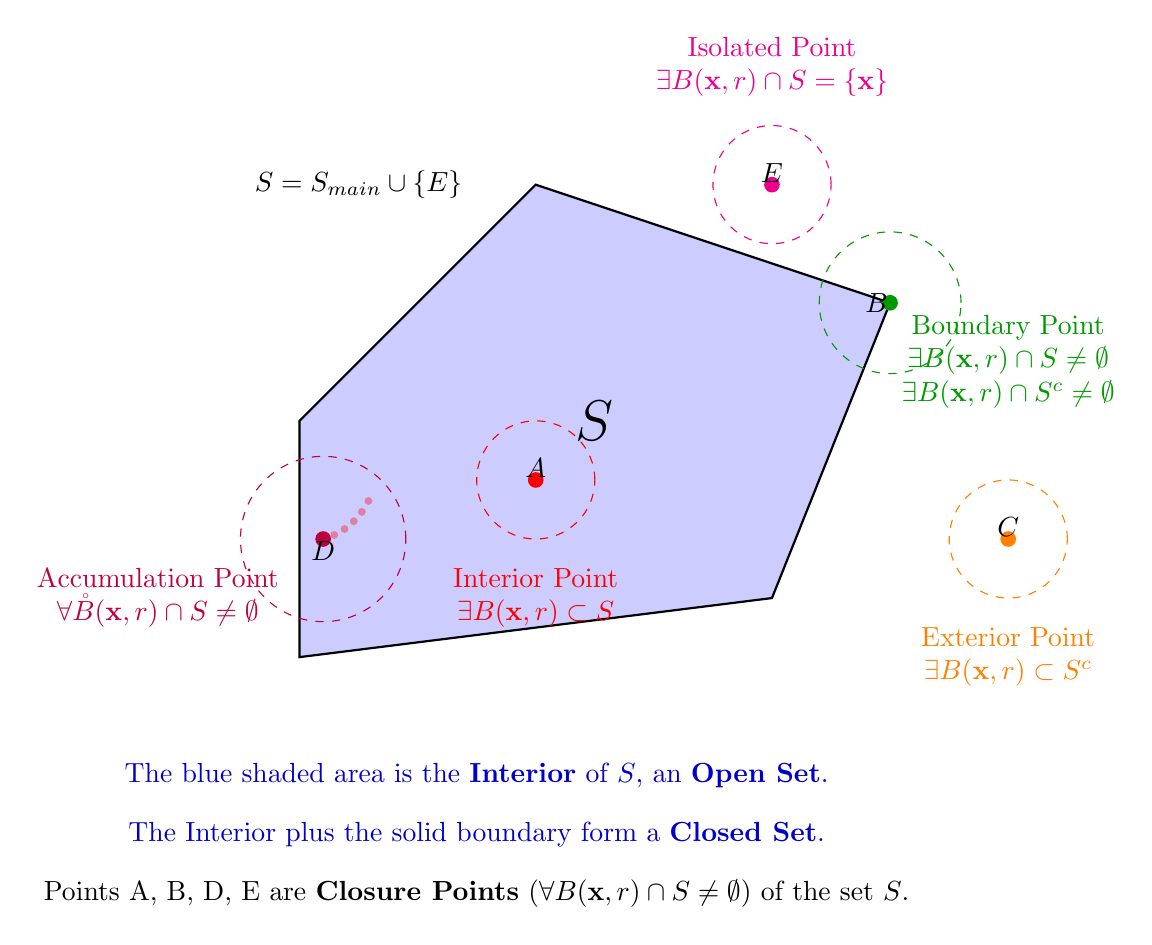
\begin{tikzpicture}[scale=1.5, every node/.style={scale=1}]

        % Define the set S
        \draw[thick, fill=blue!20] (0,0) -- (4,0.5) -- (5,3) -- (2,4) -- (0,2) -- cycle;
        \node at (2.5, 2) {\huge $S$};

        % Interior Point A
        \node[circle, fill=red, inner sep=2pt, label={[label distance=-0.2cm]90:$A$}] (A) at (2,1.5) {};
        \draw[red, dashed] (A) circle (0.5cm);
        \node[red, align=center] at (2, 0.5) {Interior Point \\ $\exists B(\mathbf{x},r) \subset S$};

        % Boundary Point B
        \node[circle, fill=green!60!black, inner sep=2pt, label={[label distance=-0.2cm]180:$B$}] (B) at (5, 3) {};
        \draw[green!60!black, dashed] (B) circle (0.6cm);
        \node[green!60!black, align=center] at (6, 2.5) {Boundary Point \\ $\exists B(\mathbf{x},r) \cap S \neq \emptyset$ \\ $\exists B(\mathbf{x},r) \cap S^c \neq \emptyset$};

        % Exterior Point C
        \node[circle, fill=orange, inner sep=2pt, label={[label distance=-0.2cm]90:$C$}] (C) at (6,1) {};
        \draw[orange, dashed] (C) circle (0.5cm);
        \node[orange, align=center] at (6, 0) {Exterior Point \\ $\exists B(\mathbf{x},r) \subset S^c$};

        % Accumulation Point D
        \node[circle, fill=purple, inner sep=2pt, label={[label distance=-0.2cm]270:$D$}] (D) at (0.2, 1) {};
        \draw[purple, dashed] (D) circle (0.7cm);
        \foreach \i in {1,...,5}{
                \node[circle, fill=purple!50, inner sep=1pt] at ($(D)+(15+5*\i:0.1*\i cm)$) {};
            }
        \node[purple, align=center] at (-1.2, 0.5) {Accumulation Point \\ $\forall \mathring{B}(\mathbf{x},r) \cap S \neq \emptyset$};

        % Isolated Point E
        % This point E belongs to the set S, which is the union of the main shape and the point E itself.
        \node[circle, fill=magenta, inner sep=2pt, label={[label distance=-0.2cm]90:$E$}] (E) at (4,4) {};
        \draw[magenta, dashed] (E) circle (0.5cm);
        \node[magenta, align=center] at (4, 5) {Isolated Point \\ $\exists B(\mathbf{x}, r) \cap S = \{\mathbf{x}\}$};
        \node at (0.5, 4) {$S = S_{main} \cup \{E\}$}; % Clarify that E is part of S

        % Annotations for Sets
        \node[blue!80!black] at (1.5,-1) {The blue shaded area is the \textbf{Interior} of $S$, an \textbf{Open Set}.};
        \node[blue!80!black] at (1.5,-1.5) {The Interior plus the solid boundary form a \textbf{Closed Set}.};
        \node at (1.5,-2) {Points A, B, D, E are \textbf{Closure Points} ($\forall B(\mathbf{x},r) \cap S \neq \emptyset$) of the set $S$.};

    \end{tikzpicture}
    \caption{Visual representation of topological points and sets. Here, the set $S$ is composed of the large shaded region (including its boundary) and the separate point E.}
    \label{fig:topology}
\end{figure}

\begin{remark*}[Accumulation \& Interior Points]
    An \textbf{interior point} must \textit{\textbf{belong to a set}} and be surrounded by a neighborhood entirely within that set,

    whereas an \textbf{accumulation point} is a point whose every neighborhood contains \textit{\textbf{at least one point from the set}}, regardless of whether it belongs to the set itself.
\end{remark*}

\begin{remark*}[Isolated \& Boundary Points]
    An \textbf{isolated point} must \textbf{belong to a set} that has a neighborhood containing no other points from that set,

    whereas a \textbf{boundary point} is a point whose every neighborhood must contain \textit{\textbf{at least one point from the set}} and \textit{\textbf{one point not from the set}}, regardless of whether it belongs to the set itself.
\end{remark*}

\section{Sequence}

\begin{definition}[Sequence]
    A \textbf{Sequence} is a \textit{function} $\{{\mathbf{x}_n}\}_{n=1}^{\infty}$ that maps natural numbers $n = 1,2,\dots$ to points in a set $S$.
\end{definition}

\begin{definition}[Converge]
    Given a metric space $(S,d)$, a sequence $\{{\mathbf{x}_n}\}_{n=1}^{\infty}$ in $S$ converges to $\mathbf{x} \in  S$ if \begin{equation*}
        \forall \epsilon >0, \exists N, \forall n > N \Rightarrow d(\mathbf{x}_n,\mathbf{x}) < \epsilon
    \end{equation*}
\end{definition}

\begin{definition}[Limit of Sequence] If a sequence converges,
    \begin{equation*}
        \lim_{n \to \infty} \mathbf{x}_n = \mathbf{x}
    \end{equation*}
\end{definition}

\begin{definition}[Set Bounded]
    A set $X \subset S$ is \textbf{bounded} if \begin{equation*}
        \exists M \in R, \mathbf{y} \in S, \forall \mathbf{x} \in X, \Rightarrow d(\mathbf{x},\mathbf{y}) < M.
    \end{equation*}
\end{definition}

\begin{definition}[Sequence Bounded]
    A sequence $\{{\mathbf{x}_n}\}_{n=1}^{\infty}$ is \textbf{bounded} if \begin{equation*}
        \exists M \in R, \mathbf{y} \in \mathbb{R}^{n}, \forall \mathbf{x}_j \in \{{\mathbf{x}_n}\}_{n=1}^{\infty}, \Rightarrow d(\mathbf{x}_j,\mathbf{y}) < M.
    \end{equation*}
\end{definition}

\begin{proposition}
    A sequence of vectors $\{{\mathbf{x}_n}\}_{n=1}^{\infty}$ in $\mathbb{R}^{m}$ converges $\iff$ all $m$ sequences of its components ($\{x_{in}\}_{n=1}^{\infty }$, for $i=1,\dots,m$) converge.
\end{proposition}


\begin{proposition} Let $\{\mathbf{x}_n\}$ be a sequence in $(S,d)$ then,
    \begin{enumerate}
        \item $\{\mathbf{x}_{n}\}$ converges to $\mathbf{x} \in S \iff \forall B(\mathbf{x},r)$ contains \textit{\textbf{nearly}} all elements of  $\{\mathbf{x}_{n}\}$, except the finite subset $\mathbf{x}_1,\dots,\mathbf{x}_M$.
        \item A sequence has at most one limit.
        \item If $\{\mathbf{x}_{n}\}$ converges, it is bounded.
    \end{enumerate}
\end{proposition}

\begin{definition}[Subsequence]
    Let $\mathcal{N} = \{n_1, n_2, \dots\}$ be an infinite subset of $\mathbb{N}$ such that $n_1 < n_2 < \dots$. A \textbf{subsequence} $\{\mathbf{y}_n\}$ of a sequence $\{\mathbf{x}_n\}$ is defined as $\mathbf{y}_j = \mathbf{x}_{n_j}$, for $j=1,2,\dots$
\end{definition}

\section{Compactness}


\begin{definition}[Open Cover]
    An \textbf{open cover} is a collection of open sets whose union contains all the elements of a given set in same space.

    For $E \subset S$, \underline{\textbf{open cover} of $E$ is $\{G_i\} \subset S$} such that $E \subset \cup_i G_i$.
\end{definition}



\begin{definition}[Subcover]
    A \textbf{subcover} is a subset of open cover which still covers $E$.
\end{definition}


\begin{definition}[Finite Subcover]
    A \textbf{finite subcover} is a subset with finite elements.

    For $E \subset S$, \underline{\textbf{finite subcover} of $E$ is indices of $\{G_{i}\} \subset S$} such that $E \subset G_{i1}  \cup \dots \cup G_{in}$.
\end{definition}


\begin{definition}
    $E \subset S$ is \textbf{compact} if \textbf{EVERY} open cover of $E$ has a \textbf{finite subcover}.
\end{definition}

\begin{example*}
    1. Any finite set is compact, such as singleton $\{\mathbf{x}\}$. 2. The interval $(0,1)$ is not compact.
\end{example*}

\begin{definition}[Sequentially Compact]
    Let $(S,d)$ be a metric space. $X \subseteq S$ is \textbf{sequentially compact} if every sequence in $X$ has a subsequence that converges to a point in $X$.

    \begin{remark*}
        The limit point must stay inside the set (this is crucial).
    \end{remark*}
    \begin{example*}
        $(0,1)$ is not sequentially compact.
    \end{example*}
\end{definition}

\begin{proposition}
    In \textbf{metric space}: \begin{equation*}
        \text{Compact} \iff \text{Sequentially compact}
    \end{equation*}
    It is not necessarily right for non-metric space.
\end{proposition}

\begin{theorem}[Heine-Borel]
    In $\mathbb{R}^{n}$ (\textbf{with the usual metric}): \begin{equation*}
        E \text{ is compact} \iff E \text{ is closed and bounded}.
    \end{equation*}
\end{theorem}

\begin{remark*}
    \textbf{With usual metric (Euclidean Space), we have:}
    \[
       \text{Closed and Bounded} \iff \text{Compact} \iff \text{Sequentially Compact}
    \]
\end{remark*}

\begin{theorem}[Bolzano-Weierstrass]
    Every \textbf{bounded} sequence in $\mathbb{R}^{n}$ (\textbf{with the usual metric}) contains a \textbf{convergent} subsequence (in $\mathbb{R}^{n}$).
\end{theorem}

\begin{proof} Proof of Bolzano-Weierstrass:
    Recursively using Bisection method.
\end{proof}

\begin{proposition}[Bolzano-Weierstrass Generalization on Set]
    $S \subset \mathbb{R}^{n}$ is \textbf{bounded} $\iff$ Every sequence in $S$ contains a \textbf{convergent} subsequence.

    \begin{remark*}
        It is actually checking if every sequence in a set fulfill the Bolzano-Weierstrass Theorem.
    \end{remark*}
\end{proposition}

\begin{theorem}
    Every bounded monotone sequence converges.
\end{theorem}

\section{Cauchy Sequences}

\begin{definition}[Cauchy Sequence]
    A sequence $\{\mathbf{x}_n\}_{n=0}^{\infty}$ in $S$ is a \textbf{Cauchy Sequence} if
    \begin{equation*}
        \forall \epsilon > 0, \exists N_{\epsilon} \Rightarrow \forall n,m>N_{\epsilon}, d(\mathbf{x}_n, \mathbf{x}_m) < \epsilon
    \end{equation*}
\end{definition}

\begin{proposition}
    Every convergent sequence is Cauchy.
\end{proposition}

\begin{remark*}
    Not all Cauchy sequences are convergent. \textbf{Remember}, the limit of convergent sequences should be in the same space. See the definition of Completeness.
\end{remark*}

\begin{lemma}
    Any Cauchy sequence is bounded.
\end{lemma}

\begin{definition}[Complete]
    A metric space $(S,d)$ is \textbf{complete} if every Cauchy sequence converges to an element in $S$.
\end{definition}

\begin{proposition}
    All compact metric spaces are complete.
\end{proposition}

\begin{remark*}
    Not every metric space is complete. e.g. the set of rational numbers $\mathbb{Q}$.\begin{align*}
         & x_1 = 1                                              \\
         & x_2 = 1.4                                            \\
         & x_3 = 1.41                                           \\
         & x_4 = 1.414                                          \\
         & \dots                                                \\
         & \lim_{n \to \infty} x_n = \sqrt{2} \notin \mathbb{Q}
    \end{align*}
\end{remark*}

\begin{proposition}
    $\mathbb{R}^{n}$ is complete.
\end{proposition}

\begin{remark*}
    Cauchy Sequence has two implications:
    \begin{itemize}
        \item to check if a sequence is convergent in a complete space,
        \item to define Completeness of a space.
    \end{itemize}
\end{remark*}


\section{Functions (from $\mathbb{R}^{n}$ to $\mathbb{R}^{m}$)}

\begin{definition}[Function and Domain]
    Let  $D \subset \mathbb{R}^{n}, n \geq 1$, and let  $\mathbb{R}^{m}$, for  $m \geq 1$.

    A \textbf{function} $f:D \subset \mathbb{R}^{n} \to \mathbb{R}^{m}$ assigns to each $\mathbf{x} \in D$ one and only one $\mathbf{y} \in \mathbb{R}^{m}$.

    $D$ is the $domain$ of the function $f$.
\end{definition}

\begin{remark*} (Categories)
    \begin{itemize}
        \item
              If \(n = 1, m = 1, f\) is a function of a real variable on a real
              variable.
        \item
              If \(n = 1, m > 1, f\) is a vector function of real values.
        \item
              If \(n > 1, m = 1, f\) is a real function of vector values.
        \item
              If \(n > 1, m > 1, f\) is a vector function of vector values.
    \end{itemize}
\end{remark*}

\section{Limit of a function}

\begin{definition}[Limits]
    Let $f: D \subset \mathbb{R}^{n} \to \mathbb{R}^{m}$. Consider
    \(\mathbf{x}_{0}\in a c c(D)\) and \(\textbf{L}\in\) \(\mathbb{R}^{m}\), $\mathbf{L}$ is the limit of if \begin{equation*}
        \forall \epsilon > 0, \exists \delta > 0, 0<||\mathbf{x} - \mathbf{x}_{0}|| < \delta \Rightarrow \left|\left|f(\mathbf{x}) - \mathbf{L}\right|\right|< \epsilon
    \end{equation*}
\end{definition}

\begin{remark*}
    The definition above is equivalent to the following:
    $\forall \epsilon > 0, \exists \delta > 0$
    \begin{itemize}
        \item $\mathbf{x} \in \mathring{B}(\mathbf{x}_0, \delta) \Rightarrow f(\mathbf{x}) \in B(\mathbf{L}, \epsilon)$,
        \item $\lim_{||\mathbf{x} - \mathbf{x}_0||\rightarrow 0}||f(\mathbf{x}) - \mathbf{L}|| = 0$.
        \item $\lim_{d(\mathbf{x},\mathbf{x}_0)\rightarrow 0}d(f(\mathbf{x}),\mathbf{L}) = 0$.
    \end{itemize}
\end{remark*}

\begin{remark*}
    How to proof the limit at \(\mathbf{x}_0\) not exists?

    Find \textbf{one} direction of the Ball that the limit not exists, e.g. \(x_1=kx_2\)
\end{remark*}

\begin{proposition}
    The limit of \(f\) at \(\mathbf{x}_0\), if it exists, is unique.
\end{proposition}

Limit Rules: Let \(f:\mathbb{R}^{n}\longrightarrow \mathbb{R}\) and\(g:\mathbb{R}^{n}\longrightarrow \mathbb{R}\) . Moreover, assume \(\lim_{\mathbf{x}\to \mathbf{x}_0}f(\mathbf{x}) = L_1\) and \(\lim_{\mathbf{x}\to \mathbf{x}_0}g(\mathbf{x}) = L_2\) ; then:
\begin{enumerate}
    \item \(\lim_{\mathbf{x}\to \mathbf{x}_0}f(\mathbf{x}) + g(\mathbf{x}) = L_1 + L_2.\)
    \item \(\lim_{\mathbf{x}\to \mathbf{x}_0}a f(\mathbf{x}) = a L_1\), for all \(a\in \mathbb{R}\).
    \item \(\lim_{\mathbf{x}\to \mathbf{x}_0}f(\mathbf{x})g(\mathbf{x}) = L_1L_2\).
    \item \(\lim_{\mathbf{x}\to \mathbf{x}_0}\frac{f(\mathbf{x})}{g(\mathbf{x})} = \frac{L_1}{L_2}\), if \(L_2\neq 0\).
    \item \(\lim_{\mathbf{x}\to \mathbf{x}_0}f(\mathbf{x})g(\mathbf{x}) = L_1^{L_2}\), (if \(L_1^{L_2}\) is well defined).
\end{enumerate}


\begin{proposition}
    \(f: \mathbb{R}^{n} \rightarrow \mathbb{R}^{m}, \mathbf{x_{0}} \in \mathbb{R}^{n}\), and \(f = (f_{1}, f_{2}, \ldots , f_{m})'\). Then, \(\forall i = 1,2, \ldots , m\)
    \[
        f(\mathbf{x}) = \mathbf{L} = \left( \begin{array}{c}L_{1} \\ L_{2} \\ \vdots \\ L_{m} \end{array} \right) \iff \lim_{\mathbf{x} \rightarrow \mathbf{x}_{0}} f_{i}(\mathbf{x}) = L_{i}
    \]
\end{proposition}


\section{Continuity}

\begin{definition}[Continuity]
    \(f: D \subset \mathbb{R}^{n} \rightarrow \mathbb{R}^{m}\) and consider \(\mathbf{x}_{0} \in D\). \(f(\mathbf{x})\) is \textbf{continuous} at \(\mathbf{x} = \mathbf{x}_0\) if \[
        \forall \epsilon > 0, \exists \delta > 0, ||\mathbf{x}-\mathbf{x_0}|| < \delta \Longrightarrow ||f(\mathbf{x}) - f(\mathbf{x}_0)|| < \epsilon
    \]
\end{definition}

\begin{remark*}
    The definition above is equivalent to the following statement:
    \[
        \forall \epsilon > 0, \exists \delta > 0, \forall\mathbf{x} \in B(\mathbf{x}_0, \delta) \Longrightarrow f(\mathbf{x}) \in B(f(\mathbf{x}_0),\epsilon).
    \]
\end{remark*}

Continuity rules: Let \(f: \mathbb{R}^{n} \rightarrow \mathbb{R}^{m}\) and
\(g: \mathbb{R}^{n} \rightarrow \mathbb{R}^{m}\). Let
\(\mathbf{x}_{0} \in \mathbb{R}^{n}\). If \(f\) and \(g\) are
continuous at \(\mathbf{x}_{0}\), then:
\begin{enumerate}
    \item
          \(f + g\) is continuous at \(\mathbf{x}_{0}\).
    \item
          \(a f\) is continuous at \(\mathbf{x}_{0}\) if \(a \in \mathbb{R}\).
    \item
          \(f \cdot g\) is continuous at \(\mathbf{x}_{0}\).
    \item
          If \(g(\mathbf{x}_{0}) \neq 0\) , then \(\frac{f}{g}\) is continuous at \(\mathbf{x}_{0}\) (when \(m = 1\)).
\end{enumerate}


\begin{proposition}
    Let \(f:\mathbb{R}^{n}\rightarrow \mathbb{R}^{m}\) \(\mathbf{x_{0}}\in \mathbb{R}^{n}\), and \(f = (f_{1},f_{2},\ldots ,f_{m})^{\prime}\). Then,

    \(f\) is continuous at \(\mathbf{x}_{0}\iff f_{i}\) is continuous at \(\mathbf{x}_{0},\forall i = 1,2,\ldots ,m.\)
\end{proposition}


\begin{proposition}
    \(f:\mathbb{R}^{n}\rightarrow \mathbb{R}^{p}\) and \(g:\mathbb{R}^{p}\rightarrow \mathbb{R}^{m}\). Let \(\mathbf{x}_0\in \mathbb{R}^n\). If \(f\) is continuous at \(\mathbf{x}_0\) and \(g\) is continuous at \(f(\mathbf{x}_0)\). Then, \(g\circ f\) is continuous at \(\mathbf{x}_0\).
\end{proposition}

\begin{remark*}
    The above propositions and rules allow us to study the continuity of numerous functions without having to resort to the definition.
\end{remark*}


\begin{definition}[Continuity on (Sub)Domain]
    Let \(A\subset \mathbb{R}^{n}\). \(f\) is continuous at \(A\) if \(\forall \mathbf{x}_0\in A\), \(f\) is continuous at \(\mathbf{x}_0\).
\end{definition}

\section{Weierstrass' Theorem}

\begin{proposition} Bounded Above and Supremum:
    \begin{itemize}
        \item If \(E \subset \mathbb{R}\) is \textbf{bounded above}, \(y = \sup E\), then \(y \in \text{cl} (E)\).
        \item If \(E \subset \mathbb{R}\) is \textbf{bounded above and closed}, then \(\sup E \in E\).
    \end{itemize}
\end{proposition}

\begin{remark*}
    Similar to infimum.
\end{remark*}

\begin{theorem}[Weierstrass Theorem]
    Suppose \textbf{\(f:X\to \mathbb{R}\) is continuous, \(X\) is compact}, and \(M = \sup_{t\in X}f(t)\), \(m = \inf_{t\in X}f(t)\). Then, there exist \(p,q\in X\) such that \(f(p) = M\) \(f(q) = m\), such that \(f(q)\leq f(x)\leq f(p)\) for all \(x\in X\).
\end{theorem}

\begin{remark*}
      The Weierstrass theorem is useful in optimization problems because it guarantees the \textbf{existence of a solution}, as long as the function being maximized/minimized is \textbf{continuous}, and the set over which it is being maximized/minimized is \textbf{closed and bounded}.
\end{remark*}


\begin{proof}[\textbf{Proof of Weierstrass Theorem}]
    Let \(\{\mathbf{y}_m\}\) be an arbitrary sequence in \(f(\mathbf{x})\).

    Consider a sequence \(\mathbf{y}_m=f(\mathbf{x}_m)\).

    Because \( X \) is compact, then \( \{\mathbf{x}_m\} \subset X \) has a convergent subsequence \( \{\mathbf{x}_{m_k}\} \), and \( \lim_{k \to \infty} \mathbf{x}_{m_k} \to \mathbf{x} \in X \). (\textbf{Bolzano Weierstrass Theorem})

    By continuity of \( f \) let \( \mathbf{y}_{m_k} = f(\mathbf{x}_{m_k}) \)
    \[
        \lim_{k \to \infty} \mathbf{y}_{m_k} = \lim_{k \to \infty} f(\mathbf{x}_{m_k}) = f(\lim_{k \to \infty} \mathbf{x}_{m_k}) = f(\mathbf{x}) = \mathbf{y}
    \]

    So \(\{\mathbf{y}_m\}\) has a convergent subsequence. Because every sequence of \(\{\mathbf{y}\}\) has a convergent subsequence, so it is \textbf{Sequentially Compact} (\textbf{Definition of Sequentially Compact}). And Since in metric space sequentially compact is equivalent to compact (\textbf{Heine-Borel Theorem}) \( \Longrightarrow \) \textbf{closed and bounded}.
\end{proof}

\newpage
\lecture{Multivariate Analysis}
% TeX root = ../Main.tex
% First argument to \section is the title that will go in the table of contents. Second argument is the title that will be printed on the page.

\section{Derivate with Direction}

\begin{definition}[Derivate with Direction]
    Let $f: D \subset  \mathbb{R}^{n} \to \mathbb{R}^{m}$. Let $\mathbf{x_0} \in int(D)$ and $\mathbf{v} \in \mathbb{R}^{n}$. The \textbf{derivative} of $f$ at point $\mathbf{x_0}$ (\textbf{with direction $\mathbf{v}$}) is:
    \[
        f'(\mathbf{x_0},\mathbf{v}) = \lim_{h \to 0} \frac{f(\mathbf{x_0}+h \mathbf{v}) - f(\mathbf{x_0})}{h}
    \]
    if the limit exists.
\end{definition}


\begin{example*}
    For $\mathbb{R}^{n} \to \mathbb{R}$ linear function $f$. We have $f'(\mathbf{x_0},\mathbf{v}) = f(\mathbf{v}).$
\end{example*}

\begin{theorem}[Mean Value Theorem]
    Let $f: \mathbb{R}^{n} \to \mathbb{R}$. Suppose $f'(\mathbf{x_0}+t \mathbf{v},\mathbf{v}) \exists \forall t \in [0,1]$. Then, $\exists \theta \in (0,1)$ such that \[
        f(\mathbf{x_0}+\mathbf{v}) - f(\mathbf{x_0}) = f'(\mathbf{x_0}+\theta \mathbf{v}, \mathbf{v}).
    \]
\end{theorem}

\section{Partial Derivative}

\begin{definition}[Partial Derivative]
    Let $f: \mathbb{R}^{n} \to \mathbb{R}$. The \textbf{partial derivative} of $f$ with $x_i$ at point $\mathbf{x_0}$ is:
    \[
        D_if(\mathbf{x_0}) = \frac{\partial f}{\partial x_i}(\mathbf{x_0}) = \lim_{h \to 0} \frac{f(\mathbf{x_0} + h \mathbf{e_i}) - f(\mathbf{x_0})}{h}
    \]
    if the limit exists.

    More generally, if $f: \mathbb{R}^{n} \to \mathbb{R}^{m} (f = (f_1, f_2, \dots,f_j,\dots,f_m)')$, the partial derivative of $f_j$ with respect to $x_i$ at $\mathbf{x_0}$ is:
    \[
        D_if_j(\mathbf{x_0}) = \frac{\partial f_j}{\partial x_i}(\mathbf{x_0}) = \lim_{h \to 0} \frac{f_j(\mathbf{x_0}_1, \dots, \mathbf{x_0}_i+h,\dots,\mathbf{x_0}_n)-f_j(\mathbf{x_0})}{h}
    \]
\end{definition}

\begin{remark*}
    Actually, the partial derivative is a derivative with direction $e_i$.
\end{remark*}
\section{Gradient}

\begin{definition}[Gradient]
    Let $f: \mathbb{R}^{n} \to \mathbb{R}$ and $\mathbf{x_0} \in \mathbb{R}^{n}$. Then the \textbf{gradient} is defined as: \[
        \nabla f(\mathbf{x_0}) = \Big(\frac{\partial f(\mathbf{x_0})}{\partial x_1}, \frac{\partial f(\mathbf{x_0})}{\partial x_2},\dots,\frac{\partial f(\mathbf{x_0})}{\partial x_n}\Big)
    \]
\end{definition}
\begin{remark*}
    The gradient is a collection of partial derivatives and described all the change rate at all axis' directions.
\end{remark*}

\section{Directional Derivative}

\begin{definition}[Directional Derivative]
    Let $f: \mathbb{R}^{n}\to \mathbb{R}^{m}, \mathbf{x_0}\in \mathbb{R}^{n}$ and $\mathbf{v}\in \mathbb{R}^{n}$ \underline{with $||\mathbf{v}||$}. Then the \textbf{directional derivative} of $f$ at $\mathbf{x_0}$ with direction $\mathbf{v}$ is given by: \[
        D_\mathbf{v}f(\mathbf{x_0}) =f'(\mathbf{x_0},\mathbf{v}) = \lim_{h \to 0} \frac{f(\mathbf{x_0+h \mathbf{v}})-f(\mathbf{x_0})}{h}
    \]
    where $h \in \mathbb{R}$ is a scalar, assuming the limit exists.
\end{definition}

\begin{remark*}
    Directional Derivative is actually a specific situation of derivative with direction when $||\mathbf{v}||=1$.

    Partial Derivate can be also seen as a special case of Directional Derivative when $\mathbf{v} = \mathbf{e_i}$.
\end{remark*}

\begin{remark*}
    Partial derivatives give the slope of the function when you move in directions parallel to the coordinate axis, i.e., when you keep all other coordinates constant with the exception of one variable.

    The notion of a directional derivative, however, allows us to compute the instantaneous rate of change of a function, i.e., when all of the variables move.
\end{remark*}

\begin{proposition}
    Let $f: \mathbb{R}^{n} \to \mathbb{R}^{m}, f_i: \mathbb{R}^{n} \to \mathbb{R}$ for $i=1,\dots,m, \mathbf{x_0} \in \mathbb{R}^{n}, \mathbf{v} \in \mathbb{R}^{n}$, then \[
        \exists f'(\mathbf{x_0}, \mathbf{v}) \iff \forall i = 1,\dots,m \quad f'_i(\mathbf{x_0},\mathbf{v})
    \]
\end{proposition}

\begin{remark*}
    Suppose $f: D \subseteq \mathbb{R}^{n} \to \mathbb{R}, \mathbf{x_0} \in \mathbb{R}^{n}$, and $\exists f'(\mathbf{x_0},\mathbf{v})$ for all $\mathbf{v} \in \mathbb{R}^{n}$. It could be the case that $f$ is not continuous at $\mathbf{x_0}$.

    Explain: all the derivative with directions are getting close to $\mathbf{x_0}$ linearly. But it could be found a non-linear direction which crosses many $\mathbf{v_i}$ make the limit varies.

    Example:
    $f(x,y) = \left\{\begin{array}{l}
            \frac{xy ^{2}}{x ^{2} + y ^{4}} \\
            0                               \\
        \end{array}\right.$
\end{remark*}


\section{Differentiability}

\begin{definition}
    Let $f: D \subseteq \mathbb{R}^{n} \to \mathbb{R}^{m}$. $f$ is \textbf{differentiable} at $\mathbf{x_0} \iff \forall \mathbf{h} \in \mathbb{R}^{n}, \exists Df(\mathbf{x_0})$ such that the following limit exists \[
        \lim_{h \to 0} \frac{||f(\mathbf{x_0}+\mathbf{h})-f(\mathbf{x_0})-Df(\mathbf{x_0})\mathbf{h}||}{||\mathbf{h}||} = 0
    \]
    where $Df(\mathbf{x_0})$ is called Jacobian Matrix.
    \begin{remark*}
        $f(\mathbf{x_0}+\mathbf{h})-f(\mathbf{x_0}) = Df(\mathbf{x_0})\mathbf{h}+g(\mathbf{h})$ with $\lim_{h \to 0} \frac{g(\mathbf{h})}{\mathbf{h}} = 0$. It's a linear approximation of $f.$
    \end{remark*}
\end{definition}

\begin{proposition}
    Let $f: D \subseteq \mathbb{R}^{n} \to \mathbb{R}^{m}$, and $\mathbf{x_0} \in \mathbb{R}^{n}$.
    $f$ is differentiable at $\mathbf{x_0} \iff f_i$ is differentiable at $\mathbf{x_0}\, \forall i = 1,\dots,m$.
\end{proposition}

\begin{proposition}
    If $f: \mathbb{R}^{n} \to \mathbb{R}$ is differentiable at $\mathbf{x_0}\in \mathbb{R}^{n}$, with differential $L_\mathbf{x_0}$, then $\forall \mathbf{v} \in \mathbb{R}^{n}, \exists f'(\mathbf{x_0}, \mathbf{v})$, in addition \[
        L_\mathbf{x_0}(\mathbf{v}) = f'(\mathbf{x_0},\mathbf{v})= \nabla f(\mathbf{x_0}) \cdot \mathbf{v}.
    \]
    , where $L_\mathbf{x_0}$ represents the linear part of the approximation $f(\mathbf{x_0}+\mathbf{h})-f(\mathbf{x_0}) = Df(\mathbf{x_0})\mathbf{h}+g(\mathbf{h})$. So we have $L_\mathbf{x_0}(\mathbf{v} + \mathbf{h})= L_\mathbf{x_0}(\mathbf{v})+L_\mathbf{x_0}(\mathbf{h})$ and $L_\mathbf{x_0}(\lambda \mathbf{v})=\lambda L_\mathbf{x_0}(\mathbf{v})$.
\end{proposition}

\begin{proof}
    If $\mathbf{v} = 0$, it is trivial that $L_{\mathbf{x_0}}(\mathbf{v}) = 0$ and $f'(\mathbf{x_0},\mathbf{v}) = 0$.

    If $\mathbf{v} \neq 0$, $f(\mathbf{x_0} + \mathbf{w}) - f(\mathbf{x_0})= L_\mathbf{x_0}(\mathbf{w}) + g(\mathbf{w}), \lim_{\mathbf{w} \to \mathbf{0}} \frac{g(\mathbf{w})}{||\mathbf{w}||} = 0$. Take $\mathbf{w} = h \mathbf{v} (h \neq 0)$, \begin{align*}
        f'(\mathbf{x_0},\mathbf{v}) = \lim_{h \to 0} \frac{f(\mathbf{x_0}+h \mathbf{v}) - f(\mathbf{x_0})}{h}
         & = \lim_{h \to 0} \frac{L_{x_0}(h \mathbf{v}) + g(h \mathbf{v})}{h}                                                                           \\
         & =\lim_{h \to 0} \frac{h L_\mathbf{x_0}(\mathbf{v})}{h} + \lim_{h \to 0} \frac{g(h \mathbf{v})}{||h \mathbf{v}||} \frac{|h|||\mathbf{v}||}{h} \\
         & = L_\mathbf{x_0}(\mathbf{v}) + ||\mathbf{v}|| \lim_{h \to 0} \frac{|h|}{h}\frac{g(h \mathbf{v})}{||h \mathbf{v}||}                           \\
         & = L_\mathbf{x_0}(\mathbf{v})
    \end{align*}
    Using $\mathbf{v} = \sum_{i=1}^{n} v_i \mathbf{e}_i$, \begin{align*}
        L_\mathbf{x_0}(\mathbf{v}) & = L_\mathbf{x_0}\Big(\sum_{i=1}^{n} v_i \mathbf{e}_i \Big) = \sum_{i=1}^{n} v_i L_\mathbf{x_0}(\mathbf{e}_i) = \sum_{i=1}^{n} v_i f'(\mathbf{x_0}, \mathbf{e}_i) = \sum_{i=1}^{n} v_i \frac{\partial f(\mathbf{x_0})}{\partial x_i} = \nabla f(\mathbf{x_0}) \cdot  \mathbf{v}
    \end{align*}
\end{proof}

\begin{remark*}
    \(D_{\mathbf{v}}f(\mathbf{x}_0) = \nabla f(\mathbf{x}_0) \cdot \mathbf{v}\). This means that, for a real-valued function, we can write the directional derivative as the inner product of the gradient and the direction.
\end{remark*}


\begin{proposition}
    Let \(f:\mathbb{R}^{n}\longrightarrow \mathbb{R}^{m}\), and \(\mathbf{x}_{0}\in \mathbb{R}^{n}\). If \(f\) is differentiable at \(\mathbf{x}_{0}\) , then it is continuous at \(\mathbf{x}_{0}\)
\end{proposition}

\begin{remark*} Summary:

    Differentiable $\Longrightarrow$ Continuous.

    Differentiable $\Longrightarrow$ Partial Derivates exist.

    Continuous $\nLeftrightarrow$ Partial Derivates exist.
\end{remark*}



\section{Jacobian Matrix and Chain Rule}

\begin{definition}
    The matrix of partial derivatives of all the $f_i$ with respect to all the $x_i$ evaluated at $\mathbf{x_0}$ is called the \textbf{Jacobian} of $\mathbf{f}$ at $\mathbf{x_0}$: \[
        \mathbf{Jf(x_0)} = \begin{pmatrix}
            \nabla f_1(\mathbf{x_0})' \\ \dots \\ \nabla f_m(\mathbf{x_0})'
        \end{pmatrix} = \begin{pmatrix}
            \frac{\partial f_1(\mathbf{x_0})}{\partial x_1} & \dots  & \frac{\partial f_1(\mathbf{x_0})}{\partial x_n} \\
            \vdots                                          & \ddots & \vdots                                          \\
            \frac{\partial f_m(\mathbf{x_0})}{\partial x_1} & \dots  & \frac{\partial f_m(\mathbf{x_0})}{\partial x_n}
        \end{pmatrix}
    \]
\end{definition}

\begin{remark*}
    If $m=n$, then the Jacobian matrix is a square matrix. We can calculate the determinant and inverse of it.
\end{remark*}

\begin{proposition}
    Let \(f: \mathbb{R}^{n} \rightarrow \mathbb{R}^{m}\) and \(g: \mathbb{R}^{m} \rightarrow \mathbb{R}^{p}\) be differentiable. Let \(f\) be continuously differentiable at some set \(U\), and \(g\) be continuously differentiable on \(f(U)\). Then, \(h: \mathbb{R}^{n} \rightarrow \mathbb{R}^{p}\), \(h(\mathbf{x}) = g[f(\mathbf{x})]\) is continuously differentiable on \(U\), with:
    \[
        D h(\mathbf{x}) = D g[f(\mathbf{x})]D f(\mathbf{x}).
    \]
\end{proposition}

\begin{remark*}
    About notation:

    If \(f: \mathbb{R}^{n} \rightarrow \mathbb{R}^{m}\) , we will denote
    \(D f(x)\mathbf{v}\) as \(\mathbf{J}f(\mathbf{x})\mathbf{v}\) while,

    if \(f: \mathbb{R}^{n} \rightarrow \mathbb{R}\) , we will denote
    \(D f(x)\mathbf{v}\) as \(\nabla f(\mathbf{x}) \cdot \mathbf{v}\) and,
    finally,

    if \(f: \mathbb{R} \rightarrow \mathbb{R}^{m}\) , we will denote
    \(D f(x)v\) as \(f'(x)v\).
\end{remark*}


\section{Additional Results}

\begin{proposition} Let \(f: \mathbb{R}^{n} \rightarrow \mathbb{R}, \mathbf{v} \in \mathbb{R}^{n}\), and \(||\mathbf{v}|| = 1\). Then
    \[
        \max_{\mathbf{v}}f^{\prime}(\mathbf{x}_{0},\mathbf{v}) = ||\nabla f(\mathbf{x}_{0})|| \quad \text{when } \mathbf{v} = \frac{\nabla f(\mathbf{x}_{0})}{||\nabla f(\mathbf{x}_{0})||},
    \]
    \[
        \min_{\mathbf{v}}f^{\prime}(\mathbf{x}_{0},\mathbf{v}) = -||\nabla f(\mathbf{x}_{0})|| \quad \text{when } \mathbf{v} = -\frac{\nabla f(\mathbf{x}_{0})}{||\nabla f(\mathbf{x}_{0})||},
    \]

    and \(\mathbf{v} \perp \nabla f(\mathbf{x}_{0}) \Rightarrow f^{\prime}(\mathbf{x}_{0}, \mathbf{v}) = 0\).
\end{proposition}

\begin{proposition}[Sufficient Condition of Differentiability]
    For function $f$, if all partial derivatives exist in $B(\mathbf{x_0},r)$, and they are continuous at $\mathbf{x_0}$, $\Longrightarrow f$ is differentiable at $\mathbf{x_0}$
\end{proposition}

\section{Level Sets (and the gradient)}


\begin{definition}
    $C_\alpha = \{\mathbf{x} \in \mathbb{R}^{n}: f(\mathbf{x}) = \alpha\}$ is a \textbf{level set} of function $f: \mathbb{R}^{n} \to \mathbb{R}$ at a given level $\alpha$.
\end{definition}

If $\mathbf{x_0}$ lies on the level set, the \textit{tangent hyperplane} to the level set is the set of all $\mathbf{x}$ that satisfy: \[
    \frac{\partial f(\mathbf{x_0})}{\partial x_1}(x_1-x_1 ^{0}) + \dots+ \frac{\partial f(\mathbf{x_0})}{\partial x_n}(x_n-x_n ^{0}) = \mathbf{0}.
\]
, which can be written as \[
    \nabla f(\mathbf{x_0}) \cdot (\mathbf{x - x_0}) = \mathbf{0}.
\]

\begin{proposition}
    $\nabla f(\mathbf{x_0})$ is orthogonal to the level set of $f$ that contains $\mathbf{x_0}$.
\end{proposition}

\begin{proof}
    To prove $\nabla f(x_0)$ is orthogonal to an arbitrary curve which passes $\mathbf{x_0}$ in level set.

    Let $f(\mathbf{x_0}) = \alpha$ and $C_\alpha = \{\mathbf{x} \in \mathbb{R}^{n}: f(\mathbf{x}) = \alpha\}$. Let $\Gamma$ be a curve within the level set of $f$ at $\alpha$, that is $\Gamma \subseteq C_\alpha$ and passed through $\mathbf{x_0}$. \[
        \mathbf{x} \in \Gamma \, \text{if } \begin{pmatrix}
            x_1 \\ \dots \\ x_n
        \end{pmatrix} = \begin{pmatrix}
            \phi_1(t) \\ \dots \\ \phi_n(t)
        \end{pmatrix} := \boldsymbol{\phi}(\mathbf{x}), \, \text{with } t \in \mathbb{R} \text{ so that } \mathbf{x_0} = \boldsymbol{\phi}(t)
    \]

    Let $g(t) = (f \circ \phi )(t) = f[\phi (t)]$, since $g(t) = a$, then \[
        g'(t) = 0 = \nabla f[\phi (t)] \cdot \phi' (t).
    \]
    In particular, when $t=t_0$, \[
        \nabla f(\mathbf{x_0}) \cdot \phi'(t_0) = 0.
    \]
\end{proof}

\section{Higher-order Derivatives}

Suppose \(f: \mathbb{R}^{n} \rightarrow \mathbb{R}^{m}\). Then \(f' : \mathbb{R}^{n} \rightarrow \mathcal{M}_{mn}\). That is, there are \(nm\) first- order partial derivatives.

Each of these has \(n\) partial derivatives, so \(f\) has \(n^{2}m\) second order partial derivatives, written \(\partial^{2}f_{k} / \partial x_{i}\partial x_{j}\), for \(k = 1, \ldots , m\) and \(i, j = 1, \ldots , n\).

We just need to stack all columns of \(f'\) and just treat it as a function from \(\mathbb{R}^{n}\) to \(\mathbb{R}^{mn}\).

If we keep on going, we will find that the vector that corresponds to \(f^{(k)}(\cdot)\) will have size \(n^{k}m\) , which grows quickly with \(k\) .


\subsection{Second-order Partial Derivatives}

\begin{definition}
    Let $f: \mathbb{R}^{n} \to \mathbb{R}$. The \textbf{second partial derivative} with respect to $x_i$ and $x_j$ at point $\mathbf{x_0}$ is \[
        D_{ij}f(\mathbf{x_0}) = \frac{\partial ^{2}f(\mathbf{x_0})}{\partial x_i \partial x_j} = \lim_{h \to 0} \frac{f'(\mathbf{x_0}+h \mathbf{e_j}, \mathbf{e_i}) - f_i(\mathbf{x_0})}{h},
    \] assuming such a limit exists.
\end{definition}


\begin{definition}
    Let \(f: D \subset \mathbb{R}^{n} \rightarrow \mathbb{R}\). We say that \(f\) is twice differentiable at \(\mathbf{x}_{0}\) if it is differentiable in an open set around \(\mathbf{x}_{0}\) (so that \(f'\) is defined in an open set around \(\mathbf{x}_{0}\)) and \(\nabla f\) is differentiable at \(\mathbf{x}_{0}\).
\end{definition}

\begin{definition}
    The \textbf{Hessian} matrix is:
    \[
        \mathbf{H}f(\mathbf{x}) = \begin{pmatrix}
            \frac{\partial ^{2}f(\mathbf{x})}{\partial x_1 \partial x_1} & \frac{\partial ^{2}f(\mathbf{x})}{\partial x_1 \partial x_2} & \dots & \frac{\partial ^{2}f(\mathbf{x})}{\partial x_1 \partial x_n} \\
            \frac{\partial ^{2}f(\mathbf{x})}{\partial x_2 \partial x_1} & \ddots                                                       &       & \frac{\partial ^{2}f(\mathbf{x})}{\partial x_2 \partial x_n} \\
            \vdots                                                       &                                                              &       & \vdots                                                       \\
            \frac{\partial ^{2}f(\mathbf{x})}{\partial x_n \partial x_1} & \dots                                                        &       & \frac{\partial ^{2}f(\mathbf{x})}{\partial x_n \partial x_n}
        \end{pmatrix}
    \]
\end{definition}

\begin{theorem}[Schwarz's - or Clairaut's- Theorem]
    If \(f\) is \(C^{2}\), then:
    \[
        \frac{\partial^{2}f(x)}{\partial x_{j}\partial x_{i}} = \frac{\partial^{2}f(x)}{\partial x_{i}\partial x_{j}}.
    \]
    It means Hessian matrix is symmetric.
\end{theorem}

\section{Taylor Formula}

\begin{theorem}
    Let \(f:D\subseteq \mathbb{R}^{n}\to \mathbb{R}\) : \(f\in C^{q}\) in \(D\) (i.e.~it has continuous derivatives up to order \(q\)). Let \(\mathbf{x},\mathbf{x_0}:[\mathbf{x_0},\mathbf{x}]\subseteq D\) and define \(\mathbf{v} = \mathbf{x} - \mathbf{x_0}\) Then, \(\exists \theta \in (0,1)\) :

    \[
        \begin{array}{rcl}{f(\mathbf{x})}&{=}&{f(\mathbf{x_0})+\sum_iD_if(\mathbf{x_0})(x_i-x_{0i})}\\{}&{}&{+\frac{1}{2}\sum_{i,j}D_{ij}f(\mathbf{x_0})(x_i-x_{0i})(x_j-x_{0j})+\cdots}\\{}&{}&{+\frac{1}{(q-1)!}\sum_{i_1\dots i_{q-1}}D_{i_1}\dots_{i_{q-1}}f(\mathbf{x_0})(x_{i_1}-x_{0i_1})\cdots(x_{i_{q-1}}-x_{0i_{q-1}})}\\{}&{}&{+\frac{1}{q!}\sum_{i_1\dots i_q}D_{i_1}\dots_{i_q}f(\mathbf{x_0}+\theta\mathbf{v})(x_{i_1}-x_{0i_1})\cdots(x_{i_q}-x_{0i_q}).}\end{array}
    \]
\end{theorem}

\begin{corollary}
    If $q = 2$, the first-order Taylor approximation is \[
        f(\mathbf{x}) = f(\mathbf{x_0}) + \nabla f(\mathbf{x_0}) \cdot (\mathbf{x - x_0}) + R_2(\mathbf{x})
    \]
\end{corollary}

\begin{corollary}
    If $q = 3$, the first-order Taylor approximation is \[
        f(\mathbf{x}) = f(\mathbf{x_0}) + \nabla f(\mathbf{x_0}) \cdot (\mathbf{x - x_0}) + \frac{1}{2}(\mathbf{x - x_0})'\mathbf{H}f(\mathbf{x_0})(\mathbf{x-x_0}) + R_3(\mathbf{x})
    \]
\end{corollary}


\section{Multiple Integrals}

\begin{theorem}[Fubini's Theorem]
    Suppose \[
        \int\int_{X \times Y} |f(x,y)|d(x,y) < \infty.
    \]
    Then,
    \[
        \int\int_{X \times Y} f(x,y)d(x,y) = \int_{Y}\left(\int_{X}f(x,y)dx\right)dy = \int_{X}\left(\int_{Y}f(x,y)dy\right)dx.
    \]
\end{theorem}

\section{Injectivity, Surjectivity, and Bijectivity}

Consider a mapping $f: A \to B$, an element of the codomain $\mathbf{y} \in B$, and the inverse image of $\mathbf{y}, f ^{-1}(\mathbf{y})$.

\begin{definition}
    A mapping $f: A \to B$ is \textbf{injective} or \textbf{one-to-one} $\iff$ \[
        \forall \mathbf{x},\mathbf{x'} \in A, f(\mathbf{x}) = f(\mathbf{x'}) \Longrightarrow \mathbf{x} = \mathbf{x'}.
    \]
\end{definition}


\begin{definition}
    A mapping $f: A \to B$ is \textbf{surjective} or \textbf{onto} $\iff$ \[
        \forall \mathbf{y} \in B, \exists \mathbf{x} \in A \Longrightarrow \mathbf{y} = f(\mathbf{x}).
    \]
\end{definition}

\begin{definition}
    A mapping $f: A \to B$ is \textbf{bijective} $iff$ it is both \textbf{injective} and \textbf{surjective}.
\end{definition}

\section{Inverse Function Theorem}

\begin{definition}
    The \textbf{identity mapping} from $A$ to $A$ is the mapping $Id_X: A \to A, Id_X(\mathbf{x}) = \mathbf{x}$.
\end{definition}

\begin{definition}
    $f$ has an \textbf{inverse} if there exists a mapping $g: B \to A$ such that $f \circ g = Id_Y$ and $g \circ f = Id_X$.
\end{definition}

\begin{proposition}
    $f$ is bijective $\iff$ $f$ has an inverse.
\end{proposition}

\begin{theorem}[Inverse Function Theorem]
    Let $f: A \subset \mathbb{R}^{n} \to B \subset \mathbb{R}^{n}$, with $A$ open. Let $\mathbf{a} \in A$ and $\mathbf{b} = f(\mathbf{a})$. Assume:
    \begin{enumerate}
        \item $f$ has all its first partial derivatives, and they are continuous in $A$; and
        \item $det[\mathbf{J}f(\mathbf{a})] \neq 0$.
    \end{enumerate}
    Then, \begin{enumerate}
        \item \textbf{the inverse function $\varphi: W \to V$ exists} (where $V, W$ are open, $\mathbf{a} \in V, \mathbf{b} \in W, \varphi (\mathbf{y}) = \mathbf{x}$),
        \item $\varphi$ is differentiable, and its differential is the inverse of $\mathbf{J}f(a)^{-1}$.
    \end{enumerate}
    In addition, if $f$ is $C ^{k}$, then $\varphi$ is also $C ^{k}$ in $W$.
\end{theorem}

\begin{remark*}
    $\forall \mathbf{x} \in A, \det (\mathbf{J}f(\mathbf{x})) \neq 0 \nRightarrow$ $f$ injective. But it could have inverse function at some local neighbor.

    \begin{example*}
        $f: A \subset \mathbb{R}^{2} \to \mathbb{R}$ with $A = \{(x_1,x_2)\in \mathbb{R}^{2}: x_1 ^{2} + x_2 ^{2} \geq 1\}$ and $f(x_1,x_2) = (x_1 ^{2} - x_2 ^{2}, x_1x_2)$.

        $\forall \mathbf{x} \in A, \det (\mathbf{J}f(\mathbf{x})) \neq 0$, but $f(1,1) = f(-1,-1)$.
    \end{example*}
\end{remark*}



\subsection{"Heuristic" argument}
\begin{align*}
     & f(\mathbf{x}) = f(\mathbf{a}) + \mathbf{J}f(\mathbf{a})(\mathbf{x} - \mathbf{a}) + R_1                                                                                                            \\
     & \mathbf{y} = f(\mathbf{a}) + \mathbf{J}f(\mathbf{a})(\mathbf{x} - \mathbf{a}) \Longrightarrow \mathbf{J}f(\mathbf{a})\mathbf{x} = \mathbf{y} - f(\mathbf{a}) + \mathbf{J}f(\mathbf{a})\mathbf{a}. \\
     & \mathbf{x} = [\mathbf{J}f(\mathbf{a})]^{-1}[\mathbf{y} - f(\mathbf{a})+\mathbf{J}f(\mathbf{a})\mathbf{a}] = \mathbf{a} + [\mathbf{J}f(\mathbf{a})]^{-1}[\mathbf{y}-f(\mathbf{a})]
\end{align*}
That's why we need $det[\mathbf{J}f(\mathbf{a})] \neq 0$.



\section{Implicit Function Theorem}

\begin{theorem}[Implicit Function Theorem]
    Let $f: \mathbb{R}^{n} \times \mathbb{R}^{m} \to \mathbb{R}^{m}, (\mathbf{x}, \mathbf{y}) \to f(\mathbf{x}, \mathbf{y})$, and let $(\mathbf{a}, \mathbf{b}) \in \mathbb{R}^{n} \times \mathbb{R}^{m}$. Assume:
    \begin{enumerate}
        \item $f(\mathbf{a}, \mathbf{b}) = \mathbf{0}$,
        \item $f$ has all its partial derivatives continuous in an open set the contains $(\mathbf{a}, \mathbf{b})$, and
        \item $\left|\frac{\partial (f_1,\dots,f_m)'}{\partial (y_1,\dots,y_m)}\right|_{(\mathbf{x,y}) = (\mathbf{a,b})} \neq 0$.
    \end{enumerate}
    Then, \begin{enumerate}
        \item \textbf{the implicit function $g: A \to B$ exists} (where $A,B$ are open, $A \subset \mathbb{R}^{n}, \mathbf{a} \in A, B \subset \mathbb{R}^{m}, \mathbf{b} \in B$, and $\forall \mathbf{x} \in A, f(\mathbf{x}, g(\mathbf{x})) = \mathbf{0}$).
        \item $g$ is continuously differentiable for all $\mathbf{x} \in A$.
    \end{enumerate}
\end{theorem}

\begin{proof}[Proof of Implicit Function Theorem]
    Define a mapping $F: \mathbb{R}^{n} \times \mathbb{R}^{m} \to \mathbb{R}^{n} \times \mathbb{R}^{m}$ such that \[
        (\mathbf{x}, \mathbf{y}) \mapsto F(\mathbf{x}, \mathbf{y}) := (\mathbf{x}, f(\mathbf{x,y}))
    \]
    That's check the two requirements of \textbf{Inverse Function Theorem} for $F$:

    1) F has all its first order partial derivatives, and they are continuous on an open set contains $(\mathbf{a, b})$. It is trivial.

    2)$\det (\mathbf{J}F) = \big|\frac{\partial (F_1,\dots,F_n,F_{n+1},\dots,F_{n+m})}{\partial (x_1,\dots,x_n,y_1,\dots,y_m)}\big|_{\mathbf{x=a,y=b}} = \begin{vmatrix}
            \boldsymbol{I_n}                                           & \boldsymbol{0}                                             \\
            \frac{\partial (f_1,\dots,f_m)'}{\partial (x_1,\dots,x_n)} & \frac{\partial (f_1,\dots,f_m)'}{\partial (y_1,\dots,y_m)}
        \end{vmatrix} = \left|\frac{\partial (f_1,\dots,f_m)'}{\partial (y_1,\dots,y_m)}\right| \neq 0$

    Specifically, there exists open $W \subseteq \mathbb{R}^{n} \times \mathbb{R}^{n}$ with $\mathbf{b} \in W$, such that $F(\mathbf{a,b}) \in W$,
    \[
        F(\mathbf{a}, \mathbf{b}) = (\mathbf{a}, f(\mathbf{a,b})) = (\mathbf{a, 0})
    \]
    Then there exists an open set in $\mathbb{R}^{n} \times \mathbb{R}^{n}$, say $A \times B \subseteq \mathbb{R}^{n} \times \mathbb{R}^{m}$ with $\mathbf{a} \in A, \mathbf{b} \in B$, such that:
    i) there exists $h: W \to A \times B$, with $h$ being the inverse function of $F$, and
    ii) $h$ is differentiable.

    Specifically, $h(\mathbf{x',y'}) = (\mathbf{x,y})$ with $F(\mathbf{x,y}) = (\mathbf{x',y'}) = (\mathbf{x, f(\mathbf{x,y})})$, which implies \[
        \left\{\begin{array}{l}
            \mathbf{x} = \mathbf{x'}      \\
            f(\mathbf{x,y}) = \mathbf{y'} \\
        \end{array}\right.
    \]
    Therefore, $h$ has to have the following form: ($f(\mathbf{x',y}) = \mathbf{y'} \Rightarrow  \mathbf{y} = k(\mathbf{x',y'})$ - inverse function) \[
        h(\mathbf{x',y'}) = (\mathbf{x'},k(\mathbf{x',y'})), \, \text{with $k$ differentiable}.
    \]

    Consider now the function $\pi : \mathbb{R}^{n} \times \mathbb{R}^{m} \to \mathbb{R}^{m}$ such that $(\mathbf{x,y}) \mapsto \pi (\mathbf{x,y}) := \mathbf{y}$. Then \[
        (\pi \circ F)(\mathbf{x,y}) = \pi [F(\mathbf{x,y})] = \pi [\mathbf{x, f(\mathbf{x,y})}] = f(\mathbf{x,y}).
    \]
    Then, for function $f[\mathbf{x}, k(\mathbf{x,y})] $ we have \[
        f[\mathbf{x}, k(\mathbf{x,y})] = f[h(\mathbf{x,y})] = (\pi \circ F)[h(\mathbf{x,y})] = \pi [(F \circ h)(\mathbf{x,y})] = \pi (\mathbf{x,y}) = \mathbf{y}
    \]

    Take $g(\mathbf{x}) = k(\mathbf{x, 0})$, then $\forall \mathbf{x} \in A$:

    1) $f(\mathbf{x},g(\mathbf{x})) = \mathbf{0}$, and

    2) $g$ is differentiable.
\end{proof}


\section{Convex Set}

\begin{definition}[Convex Set]
    Let $C \subseteq \mathbb{R}^{n}$. Then, $C$ is a \textbf{convex set} $\iff \forall \mathbf{x,y} \in C, \forall \lambda \in [0,1], \lambda \mathbf{x} + (1-\lambda)\mathbf{y} \in C$.
\end{definition}

\begin{remark*}
    $\emptyset $ and $\mathbb{R}^{n}$ are convex.
\end{remark*}

\begin{proposition}
    Let $C_i \subset \mathbb{R}^{n}$ be convex $\forall i \in \boldsymbol{I} \Longrightarrow \bigcap_{i \in I}^{}C_i$ is convex.
\end{proposition}

\begin{remark*}
    The union of convex sets is usually not convex.
\end{remark*}


\begin{definition}[Convex Linear Combination]
    Let $\mathbf{x_1, x_2, \dots, x_m} \in \mathbb{R}^{n}$ and $\lambda_1,\lambda_2,\dots,\lambda_m \in [0,1]$. Then, a \textbf{convex linear combination} of $\mathbf{x_1, x_2, \dots, x_m}$ is a vector \[
        \lambda_1 \mathbf{x_1} + \lambda_2 \mathbf{x_2} + \dots + \lambda_m \mathbf{x_m} \text{ with } \sum_{i=1}^{m} \lambda_i = 1.
    \]
\end{definition}

\begin{proposition}
    Let $C \subset \mathbb{R}^{n}$ be convex. Then any convex linear combination of the element in $C$ is in $C$.
\end{proposition}

\begin{definition}[Convex Envelope]
    Let $A = \{\mathbf{x_1, x_2, \dots,x_m}\} \subset \mathbb{R}^{n} $. The set of convex linear combination of $\mathbf{x_1, x_2, \dots,x_m}, i.e., Ec(A) = \{\sum_{i=1}^{m} \lambda_i \mathbf{x_i} : \lambda_i \in [0,1], \sum_{i=1}^{m} \lambda_i = 1, \mathbf{x_1, x_2, \dots, x_m} \in A \}$, is called \textbf{convex envelope} of $A$.
\end{definition}

\begin{remark*}
    Convex envelope is the smallest convex set which contains set $A$.
\end{remark*}

\section{Separating Hyperplane}

\begin{definition}[Hyperplane]
    A subset \(H\) of \(\mathbb{R}^{n}\) is a \textbf{hyperplane} if
    there exists \(\mathbf{a} \neq \mathbf{0} \in \mathbb{R}^{n}\) and
    \(c \in \mathbb{R}\) such that we can define the following set:
    \[
        \begin{array}{rl} & H_{a} = \{\mathbf{x} \in \mathbb{R}^{n}: a_{1} x_{1} + a_{2} x_{2} + \ldots + a_{n} x_{n} = c \} \\ & \quad = \{\mathbf{x} \in \mathbb{R}^{n}: \mathbf{a}^{\prime} \mathbf{x} = c \} . \end{array}
    \]
\end{definition}

\begin{definition}
    We can also define closed and open half- spaces:

    Closed: \(\overline{H_{a}^{+}} \equiv \left\{\mathbf{x} \in \mathbb{R}^{n}: \mathbf{a}^{\prime} \mathbf{x} \geq c \right\}\) and \(\overline{H_{a}^{- }} \equiv \left\{\mathbf{x} \in \mathbb{R}^{n}: \mathbf{a}^{\prime} \mathbf{x} \leq c \right\}\).

    Open: \(H_{a}^{+} \equiv \left\{\mathbf{x} \in \mathbb{R}^{n}: \mathbf{a}^{\prime} \mathbf{x} > c \right\}\) and \(H_{a}^{- } \equiv \left\{\mathbf{x} \in \mathbb{R}^{n}: \mathbf{a}^{\prime} \mathbf{x}< c \right\}\)
    .
\end{definition}

\begin{remark*}
    Hyperplanes and half-spaces are convex.
\end{remark*}

\begin{theorem}[Strict Separation Theorem]
    Let \(A \subset \mathbb{R}^{n}, B \subset \mathbb{R}^{n}\). If \(A, B\) are convex, \textbf{closed}, disjoint, non-empty, with \textbf{at least one of them bounded}, then \(\exists H_{a}^{+}\) and \(H_{a}^{- }\) such that \(A \subset H_{a}^{+}\) and \(B \subset H_{a}^{- }\).
\end{theorem}


\begin{theorem}[Weak Separation Theorem]
    Let \(A \subset \mathbb{R}^{n}, B \subset \mathbb{R}^{n}\). If \(A, B\) are convex, disjoint, and non-empty, then \(\exists \overline{H_{a}^{+}}\) and \(H_{a}^{- }\) such that \(A \subset \overline{H_{a}^{+}}\) and \(B \subset \overline{H_{a}^{- }}\).
\end{theorem}

\section{Convex and Concave Functions}

\begin{definition}[Convex Function]
    A convex function is defined as a function whose \textbf{area above the curve}: \(\{(\mathbf{x}, \mathbf{y}): \mathbf{y} \geq f(\mathbf{x})\}\) (called the epigraph or the hypergraph) is a \textbf{convex set}.
\end{definition}

\begin{definition}[Concave Function]
    A concave function is defined as a function whose \textbf{area below the curve}: \(\{(\mathbf{x}, \mathbf{y}): \mathbf{y} \leq f(\mathbf{x})\}\) (called the subgraph or the hypergraph) is a \textbf{convex set}.
\end{definition}

\textbf{Equivalent definitions:}

\begin{definition}[Convex Function]
    \(f\) is a convex function if \(C\) is a convex subset of \(\mathbb{R}^{n}\) and:
    \[
        \mathbf{y} \in C, \forall \lambda \in [0,1], f(\lambda \mathbf{x} + (1 - \lambda)\mathbf{y}) \leq \lambda f(\mathbf{x}) + (1 - \lambda)f(\mathbf{y})
    \]
\end{definition}

\begin{definition}[Concave Function]
    \(f\) is a concave function if \(C\) is a convex subset of \(\mathbb{R}^{n}\) and:
    \[
        \mathbf{y} \in C, \forall \lambda \in [0,1], f(\lambda \mathbf{x} + (1 - \lambda)\mathbf{y}) \geq \lambda f(\mathbf{x}) + (1 - \lambda)f(\mathbf{y})
    \]
\end{definition}

We also define strictly convex and strictly concave functions by requiring the additional condition that the inequality in the definition is strict whenever \(\mathbf{x} \neq \mathbf{y}\) and \(\lambda \in (0,1)\).

\subsection{Properties of convex and concave functions}
\begin{enumerate}
    \item
          (Sum) If \(f\) and \(g\) are convex (concave), then so is \(f + g\) .
    \item
          (Multiplication by a scalar) If \(f\) is convex (concave) and
          \(\lambda \geq 0\) , then \(\lambda f\) is convex (concave).
    \item
          Composition of functions:
          \begin{itemize}
              \item
                    If \(f\) and \(g\) are convex and \(g\) is (weakly) increasing, then
                    \(g \circ f\) is convex.
              \item
                    If \(f\) and \(g\) are concave and \(g\) is (weakly) increasing, then
                    \(g \circ f\) is concave.
          \end{itemize}
    \item
          Maximum and minimum:
          \begin{itemize}
              \item
                    If \(f\) and \(g\) are convex, then \(\max (f, g)\) is convex.
              \item
                    If \(f\) and \(g\) are concave, then \(\min (f, g)\) is concave.
          \end{itemize}
\end{enumerate}

\subsection{Characterization for differentiable functions}

\begin{proposition}
    Let \(f: C \subset \mathbb{R}^{n} \rightarrow \mathbb{R}\), with \(C\) convex. Assume that \(f\) is differentiable at \(\mathbf{x}_{0} \in \mathbb{R}^{n}\). Then:
    \begin{align*}
        f \text{(strictly) convex} \iff \forall \mathbf{x} \in \mathbb{R}^{n}, f(\mathbf{x}) & \geq f(\mathbf{x_0}) + \nabla f(\mathbf{x_0}) \cdot (\mathbf{x} - \mathbf{x_0}) \\
                                                                                             & (>)
    \end{align*}
    or
    \begin{align*}
        f \text{(strictly) concave} \iff \forall \mathbf{x} \in \mathbb{R}^{n}, f(\mathbf{x}) & \leq f(\mathbf{x_0}) + \nabla f(\mathbf{x_0}) \cdot (\mathbf{x} - \mathbf{x_0}) \\
                                                                                              & (<)
    \end{align*}
\end{proposition}

\subsection{Characterization for \(C^2\) functions}

\begin{proposition}
    Let \(f:C\subset \mathbb{R}^{n}\longrightarrow \mathbb{R}\) , with \(C\) convex and \(f\in C^{2}\) . Then:

    i) \(f\) is \textbf{convex} \(\iff \mathbf{H}f(\mathbf{x})\) is \textbf{positive} semi-definite \(\forall \mathbf{x}\in \mathbb{R}^{n}\)

    ii) \(f\) is \textbf{concave} \(\iff \mathbf{H}f(\mathbf{x})\) is \textbf{negative} semi-definite \(\forall \mathbf{x}\in \mathbb{R}^{n}\)
\end{proposition}

\begin{proposition}
    Let \(f:C\subset \mathbb{R}^{n}\longrightarrow \mathbb{R}\) , with \(C\) convex and \(f\in C^{2}\). Then:

    i) If \(\mathbf{H}f(\mathbf{x})\) is \textbf{positive} definite \(\forall \mathbf{x}\in \mathbb{R}^{n} \Longrightarrow f\) is \textbf{strictly convex}.

    ii) If \(\mathbf{H}f(\mathbf{x})\) is \textbf{negative} definite \(\forall \mathbf{x}\in \mathbb{R}^{n} \Longrightarrow f\) is \textbf{strictly concave}.
\end{proposition}

\section{Quasi-concave and Quasi-convex Functions}

\begin{definition}[Upper-level Set]
    Given a point \(a \in \mathbb{R}\), the \textbf{upper-level set} of \(f\) at level \(a\) is the set: \(\left\{\mathbf{x}: f(\mathbf{x}) \geq a\right\}\).
\end{definition}


\begin{definition}[Lower-level Set]
    Given a point \(a \in \mathbb{R}\), the \textbf{lower-level set} of \(f\) at level \(a\) is the set: \(\left\{\mathbf{x}: f(\mathbf{x}) \leq a\right\}\).
\end{definition}


\begin{definition}[Quasi-concave]
    A function is \textbf{quasi-concave} if all its upper-level sets are convex.
\end{definition}

\begin{definition}[Quasi-convex]
    A function is \textbf{quasi-convex} if all its lower-level sets are convex.
\end{definition}

\textbf{Equivalent definitions:}

\begin{definition}[Quasi-concave]
    \(f:S\subseteq \mathbb{R}^{n}\longrightarrow \mathbb{R}\) (S convex set) is quasi-concave if
    \[
        \forall \mathbf{x},\mathbf{y}\in S,\forall \lambda \in [0,1],f(\lambda \mathbf{x} + (1 - \lambda)\mathbf{y})\geq \min \{f(\mathbf{x}),f(\mathbf{y})\}
    \]
\end{definition}

\begin{definition}[Quasi-convex]
    \(f:S\subseteq \mathbb{R}^{n}\longrightarrow \mathbb{R}\) (S convex set) is quasi-convex if
    \[
        \forall \mathbf{x},\mathbf{y}\in S,\forall \lambda \in [0,1],f(\lambda \mathbf{x} + (1 - \lambda)\mathbf{y})\leq \max \{f(\mathbf{x}),f(\mathbf{y})\}
    \]
\end{definition}

We also define \textbf{strictly quasi-concave (quasi-convex) functions} by requiring the additional condition that the inequality in the definition is strict whenever \(\mathbf{x}\neq \mathbf{y}\) and \(\lambda \in (0,1)\).

\begin{remark*}Examples of Quasi-convex and Quasi-concave:

    Quasi-convex: $f(x_1,x_2) = \max(x_1, x_2)$.

    Quasi-concave: $f(x_1,x_2) = \min(x_1, x_2)$.
\end{remark*}

\subsection{Properties of quasi-concave (quasi-convex) functions}

\begin{enumerate}
    \item
          If \(f\) is quasi-concave and \(g\) increasing, then \(g \circ f\) is
          quasi-concave.
    \item
          If \(f\) is quasi-convex and \(g\) increasing, then \(g \circ f\) is
          quasi-convex.
\end{enumerate}


\newpage
\lecture{Static Optimization}
\section{Static Unconstrained Optimization}

\begin{definition}
    \[
        \min / \max_{\mathbf{x} \in B} f(\mathbf{x}).
    \]
    $f(\mathbf{x})$ is called the \textbf{objective function}. $B$ is the \textbf{constraint set} or the \textbf{feasible set}.

    $\arg \max_{\mathbf{x} \in B} f(\mathbf{x})$ represents the set of maximizers.

    $\arg \min_{\mathbf{x} \in B} f(\mathbf{x})$ represents the set of minimizers.
\end{definition}

\begin{definition}
    $f ^{*} = \max_{\mathbf{x} \in B} f(\mathbf{x})$, is the \textbf{maximum} of $f$ if $\forall \mathbf{x} \in B, f(\mathbf{x}) \leq f^{*}$, and $\exists x^{*} \in B, f(\mathbf{x^{*}}) = f ^{*}$.

    $\mathbf{x ^{*}}$ is a \textbf{maximizer} of $f$ on $B$ if $f(\mathbf{x ^{*}}) = \max_{\mathbf{x} \in B}f(\mathbf{x})$. The set of all $\mathbf{x ^{*}}$ such that $f(\mathbf{x ^{*}}) = f ^{*}$ is $\arg \max_{\mathbf{x} \in B} f(\mathbf{x})$.

    $\mathbf{x ^{*}}$ is a \textbf{strict maximizer} of $f$ on $B$ if $\forall \mathbf{x} \in B \text{ and } \mathbf{x \neq x ^{*}}, f(\mathbf{x ^{*}}) > f(\mathbf{x})$.
\end{definition}

\begin{definition}
    \(\mathbf{x}^{*}\) is a \textbf{local maximizer} if \(\exists B(\mathbf{x}^{*}, r)\) such that \(\forall \mathbf{x} \in B(\mathbf{x}^{*}, r) \cap B f(\mathbf{x}) \leq f(\mathbf{x}^{*})\).

    \(\mathbf{x}^{*}\) is a \textbf{strict local maximizer} if \(\exists B(\mathbf{x}^{*}, r)\) such that \(\forall \mathbf{x} \in B(\mathbf{x}^{*}, r) \cap B\) with \(\mathbf{x} \neq \mathbf{x}^{*}, f(\mathbf{x}) < f(\mathbf{x}^{*})\).

    \(\mathbf{x}^{*}\) is a \textbf{global maximizer} if \(\forall \mathbf{x} \in B f(\mathbf{x}) \leq f(\mathbf{x}^{*})\).

    \(\mathbf{x}^{*}\) is a \textbf{strict global maximizer} if \(\forall \mathbf{x} \in B\) with \(\mathbf{x} \neq \mathbf{x}^{*}, f(\mathbf{x}) < f(\mathbf{x}^{*})\).
\end{definition}

\subsection{First-order Conditions}

\begin{proposition}
    Let \(B\) be an open set of \(\mathbb{R}^{n}\) , and \(f: B \to \mathbb{R}\) be a differentiable function. If \(f\) has a local maximum or local minimum at \(\mathbf{x}\), then \(\nabla f(\mathbf{x}) = \mathbf{0}\), i.e., \(D_{i}f(\mathbf{x}) = \mathbf{0} \, \forall i\).
\end{proposition}

\begin{definition}
    Any point such that \(\nabla f(\mathbf{x}) = 0\) is called a \textbf{critical point} or \textbf{stationary point} of \(f\).
\end{definition}

\begin{remark*}
    If \(f\) is differentiable, then \(f\) cannot have local maxima or minima at non-critical points. Also, \(f\) might have local minima/maxima at its critical points, but it does not have to.
\end{remark*}

\begin{definition}[Saddle Point] We call $\mathbf{x_0}$ is a saddle point if
    $\forall r > 0, \exists \mathbf{x_1, x_2} \in B(\mathbf{x_0}, r) \Longrightarrow f(\mathbf{x_1}) < f(\mathbf{x_0}) < f(\mathbf{x_2})$.
\end{definition}

\subsection{Second-order Conditions}

We know that if \(\mathbf{x}^{*}\) is a critical point of the function \(f\) , then \(\nabla f(\mathbf{x}^{*}) = 0\) . To see whether \(\mathbf{x}^{*}\) is a local maximizer or minimizer, we look at \(f(\mathbf{x}^{*} + \mathbf{h})\) for some small \(\mathbf{h}\) . Now, if \(f\) is twice continuously differentiable, we can take a second-order Taylor expansion of \(f\) around \(\mathbf{x}^{*}\) to find:

\begin{proposition}
    Let \(f: B \to \mathbb{R}\) be twice continuously differentiable function on \(B\) and \(\mathbf{x}^{*}\) be a critical point in the interior of \(B\). If:

    i) \(\mathbf{H}f(\mathbf{x}^{*})\) is \textbf{negative} definite, then \(\mathbf{x}^{*}\) is a \textbf{strict local maximizer},

    ii) \(\mathbf{H}f(\mathbf{x}^{*})\) is \textbf{positive} definite, then \(\mathbf{x}^{*}\) is a \textbf{strict local minimizer},

    iii) \(\mathbf{H}f(\mathbf{x}^{*})\) is \textbf{indefinite}, then \(\mathbf{x}^{*}\) is neither a \textbf{local minimizer} nor it is a \textbf{local maximizer}, and

    iv) \(\mathbf{H}f(\mathbf{x}^{*})\) is positive semi-definite or negative semi-definite, then \(\mathbf{x}^{*}\) could be a local maximizer, local minimizer, or neither.
\end{proposition}

\begin{proposition}[not very useful]
    Let $f: B \to \mathbb{R}$ be $C ^{2}$ and $\mathbf{x ^{*}} \in int(B)$ be a local maximizer (minimizer) of $f$. Then, $\nabla f(\mathbf{x ^{*}}) = \mathbf{0}$ and $\mathbf{H}f(\mathbf{x ^{*}})$ is negative (positive) semi-definite.
\end{proposition}

\subsection{Global Maximum and minimum}

\subsubsection{Convex Optimization Problems}

\begin{definition}
    A program $\min_{\mathbf{x} \in B}f(\mathbf{x})$ is said to be a \textbf{convex program} if 1) $f$ is a convex function. 2) $B$ is a convex set.
\end{definition}

\begin{theorem}[Fundamental Theorem of Convex Programming]
    Let $\mathbf{x ^{*}}$ be a local minimizer of a convex program. Then, $\mathbf{x ^{*}}$ is a global minimizer.
\end{theorem}

\begin{proposition}
    Let $f: \mathbb{R}^{n} \to \mathbb{R}$ be a differentiable function. Then: \begin{itemize}
        \item If $f$ is convex, then $f$ has a global minimum at $\mathbf{x ^{*}} \iff \nabla f(\mathbf{x ^{*}}) = 0$, i.e., $\mathbf{x ^{*}}$ is a critical point.
        \item If $f$ is concave, then $f$ has a global maximum at $\mathbf{x ^{*}} \iff \nabla f(\mathbf{x ^{*}}) = 0$, i.e., $\mathbf{x ^{*}}$ is a critical point.
    \end{itemize}
\end{proposition}

\begin{remark*}
    If $f$ is strictly convex/concave, then $\nabla f(\mathbf{x ^{*}}) = 0$ is necessary and sufficient for $f$ to have a strict global minimum/maximum at $\mathbf{x ^{*}}$.
\end{remark*}

\begin{proposition}
    Consider a convex program, $\min_{\mathbf{x} \in B} f(\mathbf{x})$, let $C = \{\mathbf{x} \in B: \mathbf{x} \text{ are minimizers}\}$. Then $C$ is convex.
\end{proposition}

\subsection{Proof of OLS}

\begin{proof}
    The objective function is:
    \[
        \hat{\boldsymbol{\beta}} = \arg \min_{\mathbf{b}} \sum_{i=1}^{n} (y_i - \mathbf{x}'_i \mathbf{b})^{2}
    \]
    , rewrite it to matrix form, where $\mathbf{X}$ is an $n \times k$ matrix and $\mathbf{y}$ an $n \times 1$ vector:
    \[
        \hat{\boldsymbol{\beta}} = \arg \min_{\mathbf{b}} (\mathbf{y-Xb})'(\mathbf{y-Xb})
    \]
    using the fact from matrix calculus, \[
        \frac{\partial \mathbf{x'a}}{\partial \mathbf{x}} = \mathbf{a} \text{ and } \frac{\partial \mathbf{x'Ax}}{\partial \mathbf{x}} = (\mathbf{A + A'})\mathbf{x},
    \]
    and after expanding the objective function \[
        f(\mathbf{b}) = \mathbf{(y-Xb)'(y-Xb)} = \mathbf{yy'} - 2 \mathbf{b'X'y} + \mathbf{b'X'Xb},
    \]
    the corresponding first order conditions are \[
        \frac{\partial f(\mathbf{b})}{\partial \mathbf{b}} = -2 \mathbf{X'y} + 2 \mathbf{X'Xb}
    \] where $\hat{\boldsymbol{\beta}} = (\mathbf{X'X})^{-1}\mathbf{X'y}$.

    The second order conditions are \[
        \frac{\partial ^{2}f(\mathbf{b})}{\partial \mathbf{b} \partial \mathbf{b'}} = 2 \mathbf{X'X}.
    \]
    Finally, noticing that for any $\mathbf{y} \in \mathbb{R}^{k}$, $\mathbf{y'X'Xy} = \mathbf{z'z} >0 $, (with $\mathbf{z} = \mathbf{Xy}$) provided $\mathbf{z \neq 0}$, it is clear that $\mathbf{X'X}$ is positive definite (Unless there is \textbf{multicollinearity} among the regressors, i.e., $\mathbf{z = 0}$).
\end{proof}


\section{Optimization with Equality Constraints}

\subsection{The Problem}

\[
    \left\{\begin{array}{l}
        \min f(\mathbf{x})                 \\
        s.t. \, g(\mathbf{x}) = \mathbf{0} \\
    \end{array}\right.
\] where $f: D \subset \mathbb{R}^{n} \to \mathbb{R}, g: D \subset \mathbb{R}^{n} \to \mathbb{R}^{m}$, with $m < n, D$ open, and $f$ and $g$ are twice continuously differentiable.

\textbf{Assume} we can solve for $m$ elements of $\mathbf{x}$ in terms of the remaining $n-m$ i.e. \[
    g(\mathbf{x}) = \mathbf{0} \Longrightarrow \mathbf{x_B} = \boldsymbol{\varphi(x_{NB})}
\]
where $\mathbf{x = (x_B, x_{NB})}$ with $\mathbf{x_B}$ $m$-dimensional and $\mathbf{x_{NB}}$ $n-m$-dimensional.

In this case, \[
    \left\{\begin{array}{l}
        \min f(\mathbf{x})                 \\
        s.t. \, g(\mathbf{x}) = \mathbf{0} \\
    \end{array}\right. \sim \left\{\begin{array}{l}
        \min f(\mathbf{x_B}, \mathbf{x_{NB}})               \\
        s.t. \, \mathbf{x_B = \boldsymbol{\varphi}(x_{NB})} \\
    \end{array}\right.
\]
, the original problem is converted to an unconstrained optimization problem \[
    \min f(\boldsymbol{\varphi (\mathbf{x_{NB}}), \mathbf{x_{NB}}}) = F(\mathbf{x_{NB}})
\]


\subsection{Lagrange Method}
Consider
\[
    \left\{\begin{array}{l}
        \min f(x_1, x_2, x_3) \\
        s.t. \left\{\begin{array}{l}
                        g_1(x_1, x_2, x_3) = b_1 \\
                        g_2(x_1, x_2, x_3) = b_2 \\
                    \end{array}\right.
    \end{array}\right.
\]
, where $f, g_1, g_2$ are twice continuously differentiable. Moreover assume $\nabla g_1(\mathbf{x ^{*}})$ and $\nabla g_2(\mathbf{x ^{*}})$ are linearly independent(regularity condition).

Get \begin{align*}
    \frac{\partial f(\mathbf{x ^{*}})}{\partial x_1} + \frac{\partial g_1(\mathbf{x ^{*}})}{\partial x_1}\lambda_1^* + \frac{\partial g_2(\mathbf{x ^{*}})}{\partial x_1}\lambda_2 ^*=\mathbf{0} \\
    \frac{\partial f(\mathbf{x ^{*}})}{\partial x_2} + \frac{\partial g_1(\mathbf{x ^{*}})}{\partial x_2}\lambda_1^* + \frac{\partial g_2(\mathbf{x ^{*}})}{\partial x_2}\lambda_2 ^*=\mathbf{0} \\
    \frac{\partial f(\mathbf{x ^{*}})}{\partial x_3} + \frac{\partial g_1(\mathbf{x ^{*}})}{\partial x_3}\lambda_1^* + \frac{\partial g_2(\mathbf{x ^{*}})}{\partial x_3}\lambda_2 ^*=\mathbf{0}
\end{align*}


\begin{definition}
    The \textbf{Lagrangian} associated to problem $\mathcal{L}: \mathbb{R}^{n+m} \to \mathbb{R}$ is defined as \[
        \mathcal{L}(\mathbf{x,\boldsymbol{\lambda}}) = f(\mathbf{x}) + \sum_{i=1}^{m} \lambda_i g_i(\mathbf{x}) = f(\mathbf{x}) + \boldsymbol{\lambda'}g(\mathbf{x}),
    \] where $\mathbf{\lambda} = (\lambda_1, \dots, \lambda_m)'$.
\end{definition}


\subsubsection{Necessary Conditions: \textbf{Lagrange Conditions}}

\[
    \nabla f(\mathbf{x ^{*}}) + \mathbf{J}g(\mathbf{x ^{*}})'\boldsymbol{\lambda ^{*}} = \mathbf{0} \text{ and } g(\mathbf{x ^{*}}) = \mathbf{0}.
\]

\begin{definition}
    $\boldsymbol{\lambda ^{*}} = (\lambda_1, \dots, \lambda_m^*)$ is the vector of \textbf{Lagrange multiplier} associated to the respective Constraints at $\mathbf{x ^{*}}$.
\end{definition}


\subsubsection{Sufficient Conditions}

\begin{proposition}[Sufficient conditions for a strict local minimum]
    Let $\mathbf{x ^{*}}$ be a feasible point satisfying the Lagrange condition for some $\boldsymbol{\lambda ^{*}}$. Assume that the Hessian matrix of the Lagrangian function with respect to the choice variables $\mathbf{x}$, evaluated at $(\mathbf{x ^{*}, \lambda ^{*}})$,
    \[
        H_\mathbf{x}\mathcal{L}(\mathbf{x ^{*}}, \boldsymbol{\lambda ^{*}}) = \mathbf{H}f(\mathbf{x ^{*}}) + \sum_{i=1}^{m} \lambda_i ^{*}\mathbf{H}g_i(\mathbf{x ^{*}})
    \]
    is positive definite subject to the constraint $\mathbf{J}g(\mathbf{x ^{*}})\mathbf{h} = \mathbf{0}$ (specially, it is varified that $\mathbf{h'H_x\mathcal{L}(\mathbf{x ^{*}, \boldsymbol{\lambda ^{*}}})} > 0$ for all $\mathbf{h} \in  \mathbb{R}^{n}, \mathbf{h \neq 0}: \mathbf{J}g(\mathbf{x ^{*}})\mathbf{h} = \mathbf{0}$). Then $\mathbf{x}^{*}$ is a strict minimizer of $f$ subject to $g(\mathbf{x}) = \mathbf{0}$.
\end{proposition}

\begin{remark*}
    i.e., the sufficient condition is $\mathbf{h'}\mathbf{H_x}\mathcal{L}(\mathbf{x ^{*}}, \boldsymbol{\lambda})\mathbf{h} > 0, \forall \mathbf{h \neq 0}, \mathbf{J}g(\mathbf{x ^{*}})\mathbf{h} = \mathbf{0}$.
\end{remark*}

\subsection{The Convex Case}

\begin{proposition}
    If $f$ is \textbf{convex} in the feasible set of solutions $B$, and the functions $g_i, \, i=1,\dots,m$, are \textbf{linear} then the Lagrange conditions are \textbf{necessary and sufficient} for a global minimum.
\end{proposition}

\begin{proof}
    Since the Lagrange conditions are necessary for \(\mathbf{x}^{*} \in B\)
    to be a local minimizer (and, hence, global minimizer), let's show that
    they are also sufficient. To do so, let \(\mathbf{x}^{*}\), with
    associated \(\lambda^{*}\), verify the Lagrange conditions. Next,
    taking a Taylor expansion of \(f\) around \(\mathbf{x}^{*}\),
    \[
        f(\mathbf{x}) = f(\mathbf{x}^{*}) + \nabla f(\mathbf{x}^{*})\cdot (\mathbf{x} - \mathbf{x}^{*}) + \frac{1}{2} (\mathbf{x} - \mathbf{x}^{*})^{\prime}\mathbf{H}f(\pmb {\xi})(\mathbf{x} - \mathbf{x}^{*})
    \]
    with \(\xi = \mathbf{x}^{*} + \lambda \mathbf{h}\) and
    \(\lambda \in (0,1)\) . Then, since \(f\) is convex, we have
    \[
        f(\mathbf{x})\geq f(\mathbf{x}^{*}) + \nabla f(\mathbf{x}^{*})\cdot (\mathbf{x} - \mathbf{x}^{*}),
    \]
    and,
    \[
        \frac{1}{2} (\mathbf{x} - \mathbf{x}^{*})^{\prime}\mathbf{H}f(\pmb {\xi})(\mathbf{x} - \mathbf{x}^{*})\geq 0.
    \]

    Additionally, because \(\mathbf{x}^{*}\) satisfies the Lagrange
    conditions,
    \[
        \nabla f(\mathbf{x}^{*}) = -\sum_{i = 1}^{m}\lambda_{i}^{*}\nabla g_{i}(\mathbf{x}^{*}).
    \]

    Then:
    \[
        f(\mathbf{x})\geq f(\mathbf{x}^{*}) - \sum_{i = 1}^{m}\lambda_{i}^{*}\nabla g_{i}(\mathbf{x}^{*})\cdot (\mathbf{x} - \mathbf{x}^{*}).
    \]

    Finally, noticing that because the constraints are \textbf{linear},
    \[
        \nabla g_{i}(\mathbf{x}^{*})\cdot (\mathbf{x} - \mathbf{x}^{*}) = 0,\forall i = 1,\dots,m,
    \]
    we end up with \(f(\mathbf{x})\geq f(\mathbf{x}^{*})\) , as desired.
\end{proof}

\subsection{Interpretation of $\boldsymbol{\lambda ^{*}}$}
% TODO: Review this
\[
    \left\{\begin{array}{l}
        \min f(x_1, \dots, x_n) \\
        s.t. \left\{\begin{array}{l}
                        g_1(x_1, \dots, x_n) = b_1 \\
                        \qquad \quad \vdots        \\
                        g_m(x_1, \dots, x_n) = b_m \\
                    \end{array}\right.
    \end{array}\right.
\]
, with $m < n$, and $f, g$ are $C ^{2}$ in an open $D$ that contains the feasible set of solutions.

The Lagrangian $\mathcal{L}: \mathbb{R}^{n + 2m} \to \mathbb{R}$: \[
    \mathcal{L}(\mathbf{x, \boldsymbol{\lambda}, \mathbf{b}}) = f(\mathbf{x}) + \sum_{i=1}^{m} \lambda_i[g_i(\mathbf{x}) - b_i]
\]

Assume $\mathbf{(x ^{*}, \boldsymbol{\lambda ^{*}})}$ verifies both the Lagrange conditions and the sufficient conditions. In what follows, we are going to show that \[
    \lambda_j ^{*} = - \frac{\partial f(\mathbf{x ^{*}})}{\partial b_j}, \text{ for } j = 1,\dots,m.
\]

The FOCs: \begin{align*}
    \frac{\partial \mathcal{L}(\mathbf{x, \boldsymbol{\lambda}, b})}{\partial \mathbf{x}}           & = h_1(\mathbf{x, \mathcal{\lambda}, \mathbf{b}}) : \mathbb{R}^{n+2m} \to \mathbb{R}^{n} \\
    \frac{\partial \mathcal{L}(\mathbf{x, \boldsymbol{\lambda}, b})}{\partial \boldsymbol{\lambda}} & = h_2(\mathbf{x, \mathbf{b}}): \mathbb{R}^{n+m} \to \mathbb{R}^{m}                      \\
\end{align*}

For each $\mathbf{b} \in  \mathbb{R}^{n}, \mathbf{b} \in B(\mathbf{0}, r)$, from the \textbf{Implicit Function Theorem} there exist $\mathbf{x(b), \boldsymbol{\lambda}(\mathbf{b})}$ continuous and differentiable with respect to $\mathbf{b}$ at $\mathbf{b = 0}$ such that $\mathbf{x(0) = x ^{*}}$ and $\boldsymbol{\lambda(0)=\lambda ^{*}}$.

Alternatively, consider the associated Lagrangian at $\mathbf{x(b)}, \boldsymbol{\lambda(b)}$ \begin{align*}
    \mathcal{L}(\mathbf{x\boldsymbol{(\mathbf{b})}, \boldsymbol{\lambda(\mathbf{b})}, \mathbf{b}})
     & = f(\mathbf{x\boldsymbol{(\mathbf{b})}}) +
    \boldsymbol{\lambda(\mathbf{b})}\{g[\mathbf{x\boldsymbol{(\mathbf{b})}}]-\mathbf{b}\} \\
     & = f[\mathbf{x\boldsymbol{(\mathbf{b})}}]
\end{align*}

Differentiating with respect to $\mathbf{b}$,
\begin{align*}
    \frac{\partial \mathcal{L}(\mathbf{x\boldsymbol{(\mathbf{b})}, \boldsymbol{\lambda(\mathbf{b})}, \mathbf{b}})}{\partial \mathbf{b}}
     & = \nabla f[\mathbf{x\boldsymbol{(\mathbf{b})}}]\frac{\partial \mathbf{x\boldsymbol{(\mathbf{b})}}}{\partial \mathbf{b}} + \frac{\partial \boldsymbol{\lambda(\mathbf{b})}}{\partial \mathbf{b}}\{g[\mathbf{x\boldsymbol{(\mathbf{b})}}]-\mathbf{b}\} \\
     & + \boldsymbol{\lambda(\mathbf{b})}\Biggl\{\mathbf{J}g[\mathbf{x\boldsymbol{(\mathbf{b})}}]\frac{\partial \mathbf{x \boldsymbol{(\mathbf{b})}}}{\partial \mathbf{b}}- \boldsymbol{I_m}\Biggr\}                                                        \\
     & =\frac{\partial f[\mathbf{x(b)}]}{\partial \mathbf{b}}
\end{align*}

Because $\mathbf{x(b)}$ is feasible, $g[\mathbf{x\boldsymbol{(\mathbf{b})}}]-\mathbf{b = 0}$, and $\mathbf{x(b)}$ and $\boldsymbol{\lambda(\mathbf{b})}$ are solutions to the Lagrange conditions, $\nabla f[\mathbf{x \boldsymbol{(\mathbf{b})}}] + \boldsymbol{\lambda(\mathbf{b})}\mathbf{J}g[\mathbf{x\boldsymbol{(\mathbf{b})}}] = \mathbf{0}$. Therefore, substituting we obtain \[
    -\boldsymbol{\lambda(\mathbf{b})} = \frac{\partial f[\mathbf{x\boldsymbol({\mathbf{b}})}]}{\partial \mathbf{b}},
\]
which at $\mathbf{b = 0}$ implies that $\boldsymbol{\lambda ^{*}}$ is a shadow price, i.e., \[
    \boldsymbol{\lambda ^{*}} = - \frac{\partial f(\mathbf{x ^{*}})}{\partial \mathbf{b}}.
\]


\section{Static Optimization with Inequality Constraints}

\subsection{The Problem}
\[
    \left\{\begin{array}{l}
        \min f(\mathbf{x})                 \\
        s.t. g(\mathbf{x}) \leq \mathbf{0} \\
    \end{array}\right.
\]

, or \[
    \left\{\begin{array}{l}
        \min f(x_1,\dots,x_n)) \\
        s.t. \left\{\begin{array}{l}
                        g_1(x_1, \dots, x_n) \leq \mathbf{0} \\
                        \qquad \quad \vdots                  \\
                        g_m(x_1, \dots, x_n) \leq \mathbf{0} \\
                    \end{array}\right.
    \end{array}\right.
\]


\begin{definition}
    Let $\mathbf{x ^{*}}$ denote the optimizer of the problem. If $g_i(\mathbf{x ^{*}}) = \mathbf{0}$ we say that $g_i$ is \textbf{active}; in contrast, if $g_i(\mathbf{x ^{*}}) < 0$ we say that $g_i$ is \textbf{inactive}.
\end{definition}

\subsection{Kuhn-Tucker (1951)'s Conditions (Necessary Conditions)}

\begin{theorem}
    Let $\mathbf{x ^{*}}$ be a local minimizer of the problem. Moreover assume that the vectors $\nabla g_i(\mathbf{x ^{*}})$, for $j \in J = \{j: g_j(\mathbf{x ^{*}}) = \mathbf{0}\} $ are linearly independent(regularity condition). Then, there exists $\boldmath{\lambda_j ^{*}} \geq \mathbf{0}$ for $j \in J$ such that
    \[
        \nabla f(\mathbf{x ^{*}}) + \sum_{j \in J}\lambda_j^* \nabla g_j(\mathbf{x ^{*}}) = \mathbf{0}.
    \]
\end{theorem}

\begin{remark*}
    It's important to take into account that KKT works ONLY IF the regularity condition above is met.

    We should involve all the constraints in the optimality conditions:

    - for $j \notin J$, where $J = \{j: g_j(\mathbf{x ^{*}}) = \mathbf{0}\}$ we set $\lambda_j ^{*} = 0$(i.e. when $g_j(\mathbf{x ^{*}}) < 0$, we simply multiply it by zero).
\end{remark*}

\subsubsection{Alternative Formulation} \[
    \left\{\begin{array}{l}
        (1): \nabla f(\mathbf{x ^{*}}) + \sum_{j=1}^{m} \lambda_j^*\nabla g_j(\mathbf{x ^{*}}) = \mathbf{0} \\
        (2): \lambda_j^* \geq \mathbf{0} \geq \mathbf{0} \, \forall j = 1,\dots,m,                          \\
        (3): g_j(\mathbf{x ^{*}}) \leq \mathbf{0} \, \forall j = 1,\dots,m, \text{ and}                     \\
        (4): \lambda_j^*g_j(\mathbf{x ^{*}}) = \mathbf{0} \, \forall j = 1,\dots,m,
    \end{array}\right.
\]
, or (in matrix notation):
\[
    \left\{\begin{array}{l}
        (1): \nabla f(\mathbf{x ^{*}}) + \mathbf{J}g(\mathbf{x ^{*}})'\boldsymbol{\lambda ^{*}} = \mathbf{0} \\
        (2): \boldsymbol{\lambda ^{*}} \geq \mathbf{0}                                                       \\
        (3): g(\mathbf{x ^{*}}) \leq \mathbf{0}, \text{ and}                                                 \\
        (4): \boldsymbol{\lambda ^{*}} \odot g(\mathbf{x ^{*}}) = \mathbf{0}.
    \end{array}\right.
\]

\subsection{Formulation in Terms of the Lagrangian}
\[
    \left\{\begin{array}{l}
        \min f(\mathbf{x})                 \\
        s.t. g(\mathbf{x}) \leq \mathbf{0} \\
    \end{array}\right.
\]
\begin{definition}
    For the problem above, the Lagrangian is given by \[
        \boldsymbol{\mathcal{L}(\mathbf{x}, \lambda) = f(\mathbf{x}) + \lambda' g(\mathbf{x})}.
    \]

    Derivating the Lagrangian WRT $\mathbf{x}$ and $\boldsymbol{\lambda}$ we obtain \begin{align*}
         & \boldsymbol{\nabla_{\mathbf{x}}\mathcal{L}(\mathbf{x}, \lambda) = \nabla_{\mathbf{x}}f(\mathbf{x})+\mathbf{J}g(\mathbf{x})'\lambda} \\
         & \boldsymbol{\nabla_{\mathbf{\lambda}}\mathcal{L}(\mathbf{x}, \lambda) = g(\mathbf{x})}
    \end{align*}
    , so the KKT conditions can be written as \[
        \left\{\begin{array}{l}
            (1): \boldsymbol{\nabla_{\mathbf{x}}\mathcal{L}(\mathbf{x ^{*}, \lambda ^{*}})} = \mathbf{0} \\
            (2): \boldsymbol{\lambda^* \geq \mathbf{0}}                                                  \\
            (3): \boldsymbol{\nabla_{\lambda}\mathcal{L}(\mathbf{x ^{*}, \lambda ^{*}})\leq 0}           \\
            (4): \boldsymbol{\lambda ^{*} \odot \nabla_{\mathbf{\lambda}}\mathcal{L}(\mathbf{x ^{*}, \lambda*}) = 0.}
        \end{array}\right.
    \]
\end{definition}


\subsection{The Convex Case}

\begin{theorem}
    If, in addition, $f, g_{1}, \dots, g_{m}$ are convex functions, if $\mathbf{x}^{*}$ verifies the KKT conditions, then $\mathbf{x ^{*}}$ is a global minimizer.
\end{theorem}

\subsection{Sufficient Conditions}

\begin{proposition}[Sufficient conditions for a strict local minimum]
    Let $\mathbf{x ^{*}}$ be a feasible point satisfying the Lagrange condition for some $\mathbf{\lambda ^{*}}$. Assume that the Hessian matrix of the Lagrangian function WRT the choice variables $\mathbf{x}$, evaluated at $\boldsymbol{\mathbf{x}^{*},\lambda ^{*}}$,
    \[
        \boldsymbol{\mathbf{H_x}\mathcal{L}(\mathbf{x ^{*}}, \lambda ^{*}) = \mathbf{H}f(\mathbf{x ^{*}}) + \sum_{i=1}^{m} \lambda_i ^{*}\mathbf{H}g_i(\mathbf{x ^{*}})}
    \]
    is \textbf{positive definite} subject to the constraint $\boldsymbol{\mathbf{J}g_A(\mathbf{x ^{*}})\mathbf{h} = \mathbf{0}}$ for $\mathbf{h \neq 0}$, where $g_A$ denotes the active constraints at $(\mathbf{x ^{*}, \boldsymbol{\lambda ^{*}}})$ (that is, $\boldsymbol{\mathbf{h'H_x}\mathcal{L}(\mathbf{x ^{*}}, \lambda ^{*})\mathbf{h}} > 0, \forall \mathbf{h} \in \mathbb{R}^{n}, \mathbf{h \neq 0}: \boldsymbol{\mathbf{J}g_A(\mathbf{x ^{*}})\mathbf{h} = \mathbf{0}}$). Then, $\mathbf{x ^{*}}$ is a strict minimizer of $f$ subject to $g_A(\mathbf{x}) = \mathbf{0}$.
\end{proposition}

\begin{remark*}[Local Minimum]
    Change the above proposition's "\textbf{positive definite}" to "\textbf{positive semi-definite}".
\end{remark*}


\newpage
\lecture{About Exam}
\section{Analysis in $\mathbb{R}^{n}$}

Metric / Distance Function, Vector Space, Euclidean Space, Euclidean Norm, Euclidean Distance.

Open Ball, Interior Point, Exterior Point, Boundary Point, Open Set, Closed Set, Closure Point, Accumulation Point, Isolated Point.

Sequence, Sequence Converge, Sequence Bounded, Subsequence.

Compact, Sequentially Compact, \underline{$\text{Compact} \iff \text{Sequentially Compact}$}, 

\underline{$\text{Compact} \iff \text{Closed and Bounded}$}, \underline{\textbf{Bolzano-Weierstrass Theorem}}, Cauchy Sequence, Complete, \underline{$\mathbb{Q}$}.

Limits of a Function (definition, how to prove not exists), Continuity (definition, use properties to prove continuity), \underline{Weierstrass Theorem}.

\section{Multivariate Analysis}

Derivate with Direction, Partial Derivative, Gradient, Directional Derivative, Differentiable, Differential, \underline{Differential, Continuous, Partial Derivates Exist}.

Jacobian Matrix, Chain Rule, Sufficient Condition of Differentiability.

Level Set, Tangent Hyperplane.

Hessian Matrix, \textbf{Taylor Formula in $\mathbb{R}^{n}$}, Inverse Function Theorem (conditions), Implicit Function Theorem (conditions).

Convex Set, Convex Envelope, Separating Hyperplane, Strict / Weak Separation Theorem.

Convex / Concave Function (definition, properties, FOC, SOC), Upper-level / Lower-level Set, Quasi-convex / Quasi-concave Function (definition, examples, properties).


\section{Static Optimization}

\subsection{Unconstrained}
FOC (critical / stationary point, maximizer, minimizer, saddle point)
SOC (using Hessian Matrix's definiteness)
Convex Program (global maximizer and minimizer).

\subsection{Equality Constraints}
Lagrange Method, FOC, SOC, Convex Case.

\subsection{Inequality Constraints}
FOC(KKT Conditions), SOC, Convex Case.

\section{Difference and Differential Equations}

Asymptotically Stable, Unstable, Marginally Stable.

The Solutions of N-order Linear Difference Equations with Constant Coefficients.

First-order System of Difference Equations ($A(k), A$).

The Solutions of 1st-order Differential Equations (Separable, Change of variable, linear).

The Solutions of N-order Linear Differential Equations with Constant Coefficients.

First-order System of Differential Equations ($A(t), A$).




% You can add more sections here
% \section{Advanced Topic}
% 
\begin{definition}[Experiment of chance]
    It is an experiment that can be repeated under the same conditions, where the exact outcome is uncertain before it occurs, but the set of all possible outcomes is known.
\end{definition}

\begin{definition}[Probability space]
    A formal mathematical model of the experiment of chance.
\end{definition}

\begin{definition}
    The \textbf{sample space} (usually denoted by $S$ or $\Omega$) is the set of all possible outcomes of an experiment of chance.
\end{definition}
\begin{example*}
    \[
        S = \{ \text{Heads}, \text{Tails} \} \quad \text{(coin toss)}
    \]
    \[
        S = \{1, 2, 3, 4, 5, 6\} \quad \text{(roll a die)}
    \]
\end{example*}

\begin{definition}
    An \textbf{event} (denoted by $B$) is any subset of the sample space. It represents one or more outcomes of interest.
\end{definition}
\begin{example*}
    Examples (rolling a die):
    \[
        A = \{2,4,6\} \quad \text{(event: ``even number'')}
    \]
    \[
        B = \{5,6\} \quad \text{(event: ``greater than 4'')}
    \]

    Example (tossing a coin):
    \[
        C = \{\text{Heads}\} \quad \text{(event: ``get Heads'')}
    \]

\end{example*}

\subsection*{Event Space}
The \textbf{event space} (denoted by $\mathcal{B} $ or $ \mathcal{F}$) (also called a $\sigma$-algebra) is the collection of all events that are measurable in a probability model.
It must satisfy:
\begin{enumerate}
    \item $\Omega \in \mathcal{B}$ (the sample space is included),
    \item $\varnothing \in \mathcal{B}$ (the empty set is included),
    \item If $A \in \mathcal{B}$, then $A^c \in \mathcal{B}$ (closed under complementation),
    \item If $A_1, A_2, \dots \in \mathcal{B}$, then $\bigcup_{i=1}^\infty A_i \in \mathcal{B}$ (closed under countable unions).
\end{enumerate}
\begin{example*}
    Example (coin toss once):
    \[
        S = \{H, T\}, \quad
        \mathcal{B} = \{\varnothing, \{H\}, \{T\}, \{H,T\}\}
    \]
\end{example*}

\begin{definition}[A probability measure $p()$] A function which maps $B$ onto $[0,1]$ according to certain rules of Axioms of Probability.
    % Properties: \begin{enumerate}
    %     \item $ p(A) \geq 0, \forall A \in B$
    %     \item $p(\omega ) = 1$
    %     \item $\{A_i, i = 1,2,\dots\}$ be a collection of pairwise disjoint events $p(\bigcup_i A_i) = \sum_{i}^{} p(A_i)$
    %     \item 
    % \end{enumerate}
\end{definition}

\section{Random variable}

\begin{definition}
    A \textbf{random variable} $X$ can be fully characterized by means of a \textbf{cumulative distribution function (cdf)} $F_x$, a function which gives the probabilities of events of the form $X \leq x$ for all $x$. \[
        F_x : \mathbb{R} \to [0,1],\, F_X(x) \equiv p(X \leq x).
    \]
\end{definition}

Properties of a cdf: \begin{itemize}
    \item $F(-\infty ) = 0, \, F(\infty ) = 1$.
    \item $F$ is non-decreasing.
    \item $F$ is right-continuous.
\end{itemize}

\section{Discrete and continuous random variables}

\textbf{Discrete random variable}: $X$ is discrete if its range (support) is a finite or countable set. \begin{itemize}
    \item The cdf is a step function.
    \item $p(X=x_i)$ is the \textbf{probability mass function (pmf)} and $\sum_{i=1}^{} p_i = 1$.
\end{itemize}


\textbf{Continuous random variable}: The random value $X$ with cdf $F(\cdot )$ is continuous if there exists a (non-negative) function $f(\cdot )$, which is call the probability \textbf{density} function (\textbf{pdf}), such that \[
    F(x) = \int_{-\infty }^{x}f(z) \, dz
\]

Properties if the cdf and pdf of continuous random variables: \begin{itemize}
    \item $f(x) \geq 0$ at all points where $F(\cdots )$ is differentiable.
    \item $\int_{-\infty }^{\infty } f(z) \, dz = 1$.
    \item $F$ is continuous.
    \item $p(X=b) = 0$.
    \item $p(a<X<b) = \int_{a}^{b} f(z) \, dz$.
\end{itemize}

\begin{remark*}
    $f(\cdot )$ represents the probability in a unit length of interval.
    $f(\cdot )$ can be larger than $1$ in a very small interval.
\end{remark*}

\textbf{Mixed variables} \[
    F(x) = pF_d(x) + (1-p)F_c(x), \, 0 < p < 1, F_d \text{ is discrete and } F_c \text{ is continuous}
\]
\begin{remark*}
    How to understand mixed variables: Think about 2 stages:

    Wages: $20\%$ unemployed and $80\%$ employed. In those who are employed, $40\%$ worker's wages are less than $1000$, $60\%$'s wages are less than $3000$, and $100 \%$'s wages are less than $5000$. \[
        \text{wages} = \left\{\begin{array}{l}
            \text{unemployed } 20\% \Rightarrow w = 0 \\
            \text{employed } 80\% \Rightarrow \left\{\begin{array}{l}
                                                         40\% \Rightarrow 0 < w \leq 1000  \\
                                                         60\% \Rightarrow 0 < w \leq 3000  \\
                                                         100\% \Rightarrow 0 < w \leq 5000 \\
                                                     \end{array}\right.
        \end{array}\right.
    \]

    What is the probability of a random people's wage is under $3000$? We should calculate: \[
        p(w \leq 3000)  = 20\% \times 1 + 80\% \times 60\% = 68\%
    \]
\end{remark*}


\section{Univariate normal distribution}

\begin{definition}
    \textbf{Standard Normal} $N(0,1)$. \begin{itemize}
        \item pdf: $\phi (x) = \frac{1}{\sqrt{2 \pi }} \exp(-\frac{x ^{2}}{2})$ \begin{itemize}
                  \item $\phi (x) $ is symmetric about $0$.
                  \item $\phi (x) $ has a unique maximum at $x = 0$.
                  \item $\phi (x)$ has two inflexion points at $\pm 1$
              \end{itemize}
        \item cdf: $\Phi(x) = \int_{-\infty }^{x} \phi (z) \, dz$
    \end{itemize}
\end{definition}

\begin{definition}
    \textbf{Normal family} $N(\mu, \sigma^2)$. Let $Z \sim N(0,1), X \equiv \mu + \sigma Z$ with $\sigma > 0$, then $X \sim N(\mu, \sigma^2)$. \begin{itemize}
        \item cdf: $F_X(x) = \Phi(\frac{x-\mu}{\sigma})$
        \item pdf: $f_X(x) = \frac{1}{\sigma}\phi(\frac{x-\mu}{\sigma})$ \begin{itemize}
                  \item $f_X(\cdot )$ is symmetric about $\mu$.
                  \item $\phi (x) $ has a unique maximum at $x = \mu$.
                  \item $\phi (x)$ has two inflexion points at $\mu \pm \sigma$.
              \end{itemize}
    \end{itemize}
\end{definition}


\section{Functions of random variables}

\subsection{Discrete case} $y_i= g(x_i)$:
\[
    p(Y=y) = \sum_{i: g(x_i)=y}^{} p(X=x_i)
\]

\subsection{Continuous case} $Y = g(X)$, if $g$ is continuous and differentiable, $g'\neq 0$ \[
    f_Y(y) = \left| \frac{dx}{dy}\right| f_X(g^{-1}(y)) , \, \frac{dx}{dy} = \frac{1}{g'[g^{-1}(y)]}
\]

\begin{proof}
    \begin{align*}
         & F_Y(y) \equiv p(Y \leq y) = p(X \leq g^{-1}(y)) = F_X(g^{-1}(x)) \\
         & f_Y(y) = \frac{d F(x)}{dy} = \frac{dx}{dy} f_X(g^{-1}(y))
    \end{align*}
    But $\frac{dx}{dy}$ should be the absolute value because $f(\cdot) \geq 0$.
\end{proof}


\end{document}
